\chapter{Symplectic geometry}
\section{Symplectic manifolds}
\subsection{Symplectic tensors}
A $2$-covector $\omega$ on a finite-dimensional vector space $V$ is said to be \textbf{nondegenerate} if the linear map $\widehat{\omega}:V\to V^*$ defined by $\widehat{\omega}(v)=v\intprod\omega$ is invertible for every nonzero $v\in V$.

\begin{proposition}
The following are equivalent for $2$-covector $\omega$ on a finite-dimensional vector space $V$:
\begin{enumerate}
\item[(a)] $\omega$ is nondegenerate.
\item[(b)] For each nonzero $v\in V$, there exists $w\in V$ such that $\omega(v,w)\neq 0$.
\item[(c)] In terms of some $($hence every$)$ basis, the matrix $(\omega_{ij})$ representing $\omega$ is nonsingular.
\end{enumerate}
\end{proposition}
\begin{proof}
The nondegenerate condition is to say: for each nonzero $v\in V$, $v\intprod\omega\neq0$, which is exactly (b). Now let $(E_1,\dots,E_n)$ be a basis of $V$, and $W=(\omega_{ij})$ be the matrix. Then for $v=v^iE_i$ and $w=w^jE_j$,
\[\omega(v,w)=\omega_{ij}v^iw^j.\]
Thus
\begin{align*}
\omega(v,w)=0\text{ for all $w\in V$}\iff \omega_{ij}v^i=0\text{ for all $j$}\iff\text{$v$ is a solution of $W^TX=0$}.
\end{align*}
so $\omega$ is nondegenerate if and only if $W$ is nonsingular.
\end{proof}

A nondegenerate $2$-covector is called a \textbf{symplectic tensor}. A vector space $V$ endowed with a specific symplectic tensor is called a \textbf{symplectic vector space}.

\begin{example}\label{symplectic tensor eg}
Let $V$ be a $2n$-dimensional vector space. Let $(A_1,\dots,A_n,B_1,\dots,B_n)$ be a basis of $V$ and $(\alpha^1,\dots,\alpha^n,\beta^1,\dots,\beta^n)$ denote the corresponding dual basis for $V^*$, and let $\omega\in\bigwedge^2(V^*)$ be the $2$-covector defined by
\begin{align}\label{symplectic tensor-1}
\omega=\sum_{i=1}^{n}\alpha^i\wedge\beta^i.
\end{align}
Note that the action of $\omega$ on basis vectors is given by
\begin{align}\label{symplectic tensor-2}
\omega(A_i,A_j)=\omega(B_i,B_j)=0,\quad \omega(A_i,B_j)=-\omega(B_j,A_i)=\delta_{ij}.
\end{align}
and the matrix $(\omega_{ij})$ representing $\omega$ is
\[\begin{pmatrix}
0&I_n\\
-I_n&0
\end{pmatrix}\]
Thus $\omega$ is nondegenerate, and so is a symplectic tensor.
\end{example}

If $(V,\omega)$ is a symplectic vector space and $S\sub V$ is any linear subspace, we define the \textbf{symplectic complement} of $S$, denoted by $S^\bot$, to be the subspace
\[S^\bot=\{v\in V:\omega(v,w)=0\text{ for all $w\in S$}\}.\]
As the notation suggests, the symplectic complement is analogous to the orthogonal complement in an inner product space. Just as in the inner product case, the dimension of $S^\bot$ is the codimension of $S$, as the next lemma shows.

\begin{lemma}\label{symplectic complement dim}
Let $(V,\omega)$ be a symplectic vector space. For any linear subspace
$S\sub V$, we have $\dim S+\dim S^\bot=\dim V$.
\end{lemma}
\begin{proof}
Let $S\sub V$ be a subspace, and define a linear map $\varPhi:V\to S^*$ by $\varPhi(v)=(v\intprod\omega)|_S$, or equivalently
\[\varPhi(v)(w)=\omega(v,w).\]
Suppose $\varphi$ is an arbitrary element of $S^*$, and let $\widetilde{\varphi}\in V^*$ be any extension of $\varphi$ to a linear functional on all of $V$. Since the map $\widehat{\omega}:V\to V^*$ is an isomorphism, there exists $v\in V$ such that $v\intprod\omega=\widetilde{\varphi}$. It follows that $\varPhi(v)=\varphi$, and therefore $\varPhi$ is surjective. By the rank-nullity law, $S^\bot=\ker\varPhi$ has dimension equal to $\dim V-\dim S^*=\dim V-\dim S$.
\end{proof}

\begin{proposition}
Let $(V,\omega)$ be a symplectic vector space and $S\sub V$ be a linear subspace. Then $(S^\bot)^\bot=S$.
\end{proposition}
\begin{proof}
By definition, since $\omega(v,w)=-\omega(w,v)$, we have $S\sub(S^\bot)^\bot$. Now note that
\[\dim(S^\bot)^\bot=\dim V-\dim S^\bot=\dim S,\]
thus $(S^\bot)^\bot=S$.
\end{proof}

Symplectic complements differ from orthogonal complements in one important respect: although it is always true that $S\cap S^\bot=0$ in an inner product space, this need not be true in a symplectic vector space. Indeed, if $S$ is $1$-dimensional, the fact that $\omega$ is alternating forces $\omega(v,v)=0$ for every $v\in S$, so $S=S^\bot$. Carrying this idea a little further, a linear subspace $S\sub V$ is said to be
\begin{itemize}
\item \textbf{symplectic} if $S\cap S^\bot=\{0\}$.
\item \textbf{isotropic} if $S\sub S^\bot$.
\item \textbf{coisotropic} if $S\sups S^\bot$.
\item \textbf{Lagrangian} if $S=S^\bot$.
\end{itemize}

\begin{proposition}\label{symplectic subspace iff}
Let $(V,\omega)$ be a symplectic vector space and $S\sub V$ be a linear subspace. Then
\begin{enumerate}
\item[(a)] $S$ is symplectic if and only if $S^\bot$ is symplectic.
\item[(b)] $S$ is symplectic if and only if $\omega|_S$ is nondegenerate.
\item[(c)] $S$ is isotropic if and only if $\omega|_S=0$.
\item[(d)] $S$ is coisotropic if and only if $S^\bot$ is isotropic.
\item[(e)] $S$ is Lagrangian if and only if $\omega|_S=0$ and $\dim S=\frac{1}{2}\dim V$.
\end{enumerate}
\end{proposition}
\begin{proof}
Since $(S^\bot)^\bot=S$, part (a) and (d) are immediate. Next, we note that
\[\text{$v\in S\cap S^\bot$}\iff\text{$\omega(v,w)=0$ for all $w\in S$}.\]
Thus $S$ is symplectic if and only if $\omega|_S$ is nondegenerate, and $S$ is isotropic if and only if $\omega|_S=0$.\par
Finally, $S$ is Lagrangian means $S$ and $S^\bot$ are both isotropic, which implies $\omega|_S=0$ and $\dim S=\frac{1}{2}\dim V$. Conversely, if $S$ is isotropic and $\dim S=\frac{1}{2}\dim V$, then
$S\sub S^\bot$ with $\dim S=\dim S^\bot$. Thus $S=S^\bot$ and $S$ is Lagrangian. 
\end{proof}

The symplectic tensor $\omega$ defined in \cref{symplectic tensor eg} turns out to be the prototype of all symplectic tensors, as the next proposition shows. This can be viewed as a symplectic version of the Gram-Schmidt algorithm.

\begin{proposition}[\textbf{Canonical Form for a Symplectic Tensor}]\label{symplectic tensor canonical form}
Let $\omega$ be a symplectic tensor on an $m$-dimensional vector space $V$. Then $V$ has even dimension $m=2n$, and there exists a basis for $V$ in which $\omega$ has the form $(\ref{symplectic tensor-1})$.
\end{proposition}
\begin{proof}
The tensor $\omega$ has the form $(\ref{symplectic tensor-1})$ with respect to a basis $(A_1,\dots,A_n,B_1,\dots,B_n)$ if and only if its action on basis vectors is given by $(\ref{symplectic tensor-2})$.We prove the theorem by induction on $m=\dim V$ by showing that there is a basis with this property.\par
For $m=0$ there is nothing to prove. Suppose $(V,\omega)$ is a symplectic vector space of dimension $m=1$, and assume that the proposition is true for all symplectic vector spaces of dimension less than $m$. Let $A_1$ be any nonzero vector in $V$. Since $\omega$ is nondegenerate, there exists $B_1\in V$ such that $\omega(A_1,B_1)\neq0$. Multiplying $B_1$ by a constant if necessary, we may assume that $\omega(A_1,B_1)=1$. Because $\omega$ is alternating, $B_1$ cannot be a multiple of $A_1$, so the set $\{A_1,B_1\}$ is linearly independent, and hence $\dim V\geq2$.\par
Let $S\sub V$ be the span of $\{A_1,B_1\}$. Then $\dim S^\bot=\dim m-2$ by \cref{symplectic complement dim}. Since $\omega|_S$ is nondegenerate, by \cref{symplectic subspace iff} it follows that $S$ is symplectic, and thus $S^\bot$ is also symplectic. By induction, $S^\bot$ is even-dimensional and there is a basis $(A_2,\dots,A_n,B_2,\dots,B_n)$ for $S^\bot$ such that $(\ref{symplectic tensor-2})$ is satisfied for $2\leq i,j\leq n$. It follows easily that $(A_1,\dots,A_n,B_1,\dots,B_n)$ is the required basis for $V$.
\end{proof}

Because of this, if $(V,\omega)$ is a symplectic vector space, a basis $(A_1,\dots,A_n,B_1,\dots,B_n)$ for $V$ is called a \textbf{symplectic basis} if $(\ref{symplectic tensor-2})$ holds, which is equivalent to $\omega$ being given by $(\ref{symplectic tensor-1})$ in terms of the dual basis. The proposition then says that every symplectic vector space has a symplectic basis.\par
This leads to another useful criterion for $2$-covector to be nondegenerate. For an alternating tensor $\omega$, the notation $\omega^k$ denotes the $k$-fold wedge product $\omega\wedge\cdots\wedge\omega$.

\begin{proposition}\label{symplectic tensor iff n-fold product nonzero}
Suppose $V$ is a $2n$-dimensional vector space and $\omega\in\bigwedge^2(V^*)$. Then $\omega$ is a symplectic tensor if and only if $\omega^n\neq 0$.
\end{proposition}
\begin{proof}
Suppose first that $\omega$ is a symplectic tensor. Let $(A_i,B_i)$ be a symplectic basis for $V$, and write $\omega=\sum_{i=1}^{n}\alpha^i\wedge\beta^i$ in terms of the dual coframe. Then we compute
\[\omega^n=\sum'_{I}\alpha^{i_1}\wedge\beta^{i_1}\wedge\cdots\wedge\alpha^{i_n}\wedge\beta^{i_n}=n!(\alpha^1\wedge\beta^1\wedge\cdots\wedge\alpha^n\wedge\beta^n)\neq 0.\]

Conversely, suppose $\omega$ is degenerate. Then there is a nonzero vector $v\in V$ such that $v\intprod\omega=\widehat{\omega}(v)=0$. Since interior multiplication by $v$ is an antiderivation, by induction we can show
\[v\intprod(\omega^n)=n(v\intprod\omega)\wedge\omega^{n-1}=0.\]
We can extend $v$ to a basis $(E_1,\dots,E_{2n})$ for $V$ with $E_1=v$, and then $\omega^n(E_1,\dots,E_{2n})=0$, which implies $\omega^n=0$.
\end{proof}

\subsection{Symplectic structures on manifolds}
Now let us turn to a smooth manifold $M$. A \textbf{nondegenerate $2$-form} on $M$ is a $2$-form $\omega$ such that $\omega_p$ is a nondegenerate $2$-covector for each $p\in M$. A \textbf{symplectic form} on $M$ is a closed nondegenerate $2$-form. A smooth manifold endowed with a specific choice of symplectic form is called a \textbf{symplectic manifold}. A choice of symplectic form is also sometimes called a \textbf{symplectic structure}.

If $(M_1,\omega_1)$ and $(M_2,\omega_2)$ are symplectic manifolds, a diffeomorphism $F:M_1\to M_2$ satisfying $F^*\omega_2=\omega_1$ is called a \textbf{symplectomorphism}. The study of properties of symplectic manifolds that are invariant under symplectomorphisms is known as symplectic geometry or symplectic topology.

\begin{example}[\textbf{Examples of Symplectic Manifolds}]
\mbox{}
\begin{enumerate}
\item[(a)] With standard coordinates on $\R^{2n}$ denoted by $(x^1,\dots,x^n,y^1,\dots,y^n)$, the $2$-form
\[\omega=\sum_{i=1}^{n}dx^i\wedge dy^i\]
is symplectic: it is obviously closed, and it is nondegenerate because its value at each point is the symplectic tensor of \cref{symplectic tensor eg}. This is called the \textbf{standard symplectic form} on $\R^{2n}$.
\item[(b)] Suppose $\Sigma$ is any orientable smooth $2$-manifold and $\omega$ is a nonvanishing smooth $2$-form on $\omega$. Then $\omega$ is closed because $d\omega$ is a $3$-form on a $2$-manifold.
Moreover, in two dimensions every nonvanishing $2$-form is nondegenerate (by \cref{symplectic tensor iff n-fold product nonzero}), so $(\Sigma,\omega)$ is a symplectic manifold.
\end{enumerate}
\end{example}

Suppose $(M,\omega)$ is a symplectic manifold. An (immersed or embedded) submanifold $S\sub M$ is said to be a \textbf{symplectic}, \textbf{isotropic}, \textbf{coisotropic}, or \textbf{Lagrangian} submanifold if $T_pS$ (thought of as a subspace of $T_pM$) has the corresponding property at each point $p\in S$. More generally, a smooth immersion (or embedding) $F:N\to M$ is said to have one of these properties if the subspace $dF_p(T_pN)\sub T_{F(p)}M$ has the corresponding property for every $p\in N$. Thus a submanifold is symplectic (isotropic, etc.) if and only if its inclusion map has the same property.

\begin{proposition}\label{symplectic isotropic map iff pullback}
Suppose $(M,\omega)$ is a symplectic manifold and $F:N\to M$ is a smooth immersion. Then $F$ is isotropic if and only if $F^*\omega=0$, and $F$ is symplectic if and only if $F^*\omega$ is a symplectic form.
\end{proposition}
\begin{proof}
By \cref{symplectic subspace iff}, $F$ is isotropic means $\omega|_{dF(TN)}=0$, which means for all $v,w\in T_pN$ we have
\[0=\omega(dF_p(v),dF_p(w))=F^*\omega(v,w).\]
So Therefore $F$ is isotropic if and only if $F^*\omega=0$ on $N$. Similarly, by \cref{symplectic subspace iff} we can show that $F$ is symplectic if and only if $F^*\omega$ is nondegenerate on $N$, which is to say $F^*\omega$ is a symplectic form.
\end{proof}

\paragraph{The canonical symplectic form on the cotangent bundle}
The most important symplectic manifolds are total spaces of cotangent bundles, which carry canonical symplectic structures that we now define. First, there is a natural $1$-form $\tau$ on the total space of $T^*M$, called the \textbf{tautological $\bm{1}$-form}, defined as follows. A point in $T^*M$ is a covector $\varphi\in T_q^*M$ for some $q\in M$, we denote such a point by the notation $(q,\varphi)$. We define $\tau\in\Omega^1(T^*M)$ (a $1$-form on the total space of $T^*M$) by
\[\tau_{(q,\varphi)}=d\pi^*_{(q,\varphi)}\varphi.\]
where $\pi:T^*M\to M$ is the projection. In other words, the value of $\tau$ at $(q,\varphi)$ is the pullback with respect to $\pi$ of the covector $\varphi$ itself. If $v$ is a tangent vector in $T_{(q,\varphi)}(T^*M)$, then
\begin{align}\label{tautological form def}
\tau_{(q,\varphi)}(v)=\varphi\big(d\pi_{(q,\varphi)}(v)\big).
\end{align}

\begin{proposition}\label{tautological form symplectic}
Let $M$ be a smooth manifold. The tautological $1$-form $\tau$ is smooth, and $\omega=-d\tau$ is a symplectic form on the total space of $T^*M$.
\end{proposition}
\begin{figure}[htbp]
\centering
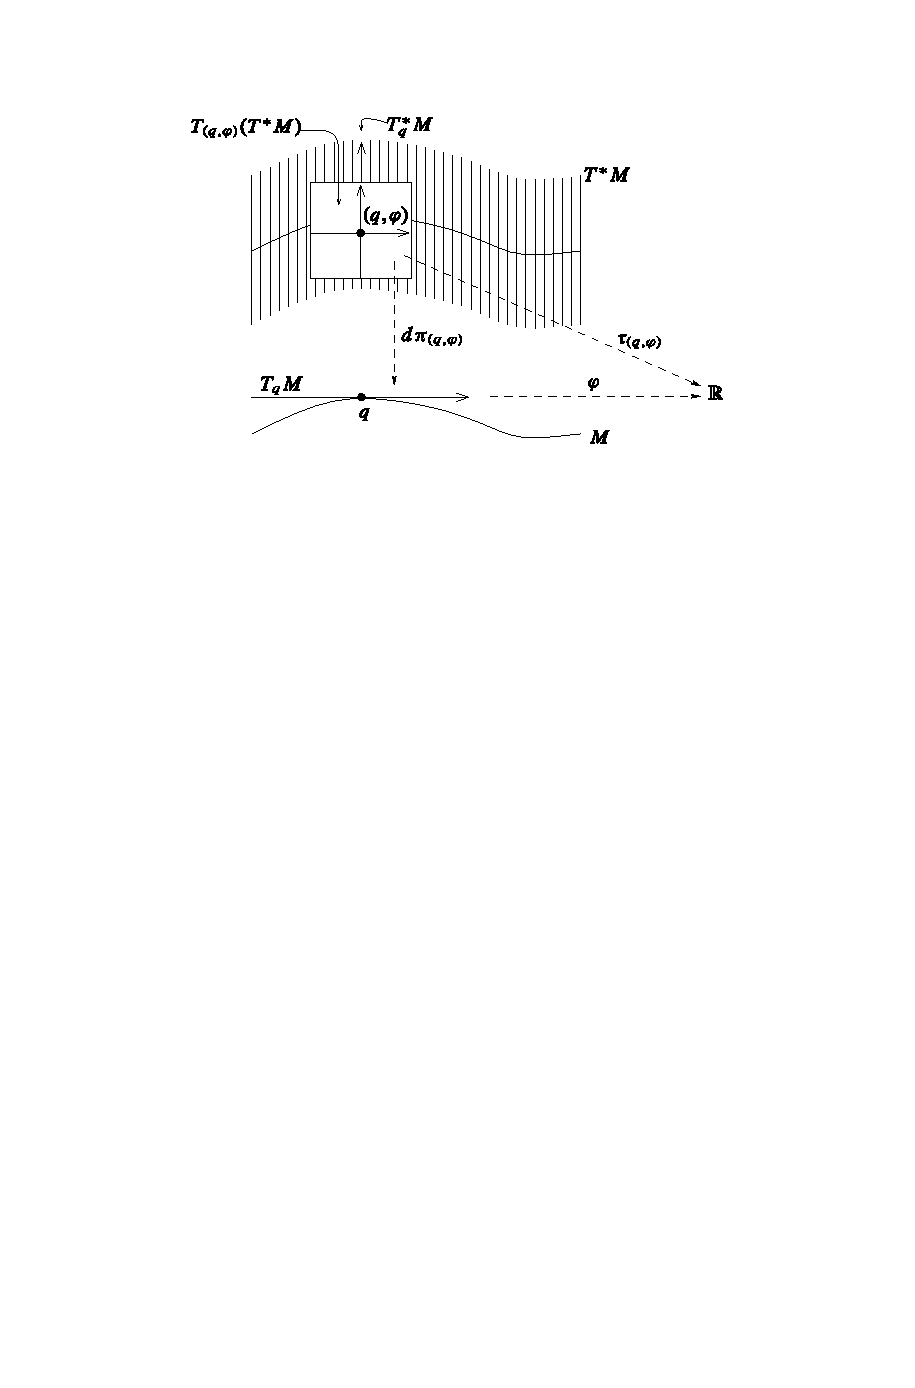
\includegraphics{pictures/tautological-form}
\caption{The tautological $1$-form on $T^*M$.}
\end{figure}
\begin{proof}
Let $(x^i)$ be smooth coordinates on $M$, and let $(x^i,\xi_i)$ denote the corresponding natural coordinates on $T^*M$. Recall that the coordinates of $(q,\varphi)\in T^*M$ are defined to be $(x^i,\xi_i)$, where $(x^i)$ is the coordinate representation of $q$, and $\xi_idx^i$ is the coordinate representation of $\varphi$. In terms of these coordinates, the projection $\pi:T^*M\to M$ has the coordinate expression $\pi(x,\xi)=x$. This implies that $d\pi^*(dx^i)=dx^i$, so the coordinate expression for $\tau$ is
\[\tau_{(x,\xi)}=d\pi^*_{(x,\xi)}(\xi_idx^i)=\xi_idx^i.\]
It follows immediately that $\tau$ is smooth, because its component functions in these coordinates are linear.\par
Let $\omega=-d\tau\in\Omega^2(T^*M)$. Clearly, $\omega$ is closed, because it is exact. Moreover, in natural coordinates,
\[\omega=\sum_{i=1}^{n}dx^i\wedge d\xi_i.\]
Under the identification of an open subset of $T^*M$ with an open subset of $\R^{2n}$ by means of these coordinates, $\omega$ corresponds to the standard symplectic form on $\R^{2n}$. It follows that $\omega$ is symplectic.
\end{proof}

The symplectic form defined in this proposition is called the canonical symplectic form on $T^*M$. One of its many uses is in giving the following somewhat more geometric interpretation of what it means for a $1$-form to be closed.

\begin{proposition}\label{Symplectic manifold one form is embedding to T^*}
Let $M$ be a smooth manifold, and let $\sigma$ be a smooth $1$-form on $M$. Thought of as a smooth map from $M$ to $T^*M$, $\sigma$ is a smooth embedding, and $\sigma$ is closed if and only if its image $\sigma(M)$ is a Lagrangian submanifold of $T^*M$.
\end{proposition}
\begin{proof}
Throughout this proof we need to remember that  $\sigma:M\to T^*M$ is playing two roles: on the one hand, it is a $1$-form on $M$, and on the other hand, it is a smooth map between manifolds. Since they are literally the same map, we do not use different notations to distinguish between them.\par
In terms of smooth local coordinates $(x^i)$ for $M$ and corresponding natural coordinates $(x^i,\xi_i)$ for $T^*M$, the map $\sigma:M\to T^*M$ has the coordinate representation
\[\sigma(x^1,\dots,x^n)=(x^1,\dots,x^n,\sigma_1(x),\dots,\sigma_n(x)),\]
where $\sigma_idx^i$ is the coordinate representation of $\sigma$ as a $1$-form. It follows immediately that $\sigma$ is a smooth immersion, and it is injective because 
$\pi\circ\sigma=\mathrm{id}_M$. To show that it is an embedding, it suffices by \cref{smooth embedd if} to show that it is a proper map. This in turn follows from the fact that $\pi$ is a left inverse for $\sigma$, by \cref{proper map if}.\par
Because $\sigma(M)$ is $n$-dimensional, it is Lagrangian if and only if it is isotropic, which is the case if and only if  $\sigma^*\omega=0$ (\cref{symplectic isotropic map iff pullback}). The pullback of the tautological form $\tau$ under $\sigma$ is
\[\sigma^*\tau=\sigma^*(\xi_idx^i)=\sigma_idx^i=\sigma.\]
This can also be seen somewhat more invariantly from the computation
\[(\sigma^*\tau)_p(v)=\tau_{\sigma(p)}\big(d\sigma_p(v)\big)=\sigma_p\big(d\pi_{\sigma(p)}\circ d\sigma_p(v)\big)=\sigma_p(d(\pi\circ\sigma)_p(v))=\sigma_p(v).\]
which follows from the definition of $\tau$ and the fact that $\pi\circ\sigma=\mathrm{id}_M$. Therefore,
\[\sigma^*\omega=-\sigma^*d\tau=-d(\sigma^*\tau)=-d\sigma.\]
It follows that $\sigma$ is a Lagrangian embedding if and only if $d\sigma=0$.
\end{proof}

\begin{proposition}\label{submani of T^*M is section iff}
Let $M$ be a smooth manifold, and let $S$ be an embedded Lagrangian submanifold of the total space of $T^*M$.
\begin{enumerate}
\item[(a)] If $S$ is transverse to the fiber of $T^*M$ at a point $q\in T^*M$, then there exist a neighborhood $V$ of $q$ in $S$ and a neighborhood $U$ of $\pi(q)$ in $M$ such that $V$ is the image of a smooth closed $1$-form defined on $U$.
\item[(b)] $S$ is the image of a globally defined smooth closed $1$-form on $M$ if and only if $S$ intersects each fiber transversely in exactly one point.
\end{enumerate}
\end{proposition}
\begin{proof}
If $S$ is transverse to the fiber of $T^*M$ at a point $q\in T^*M$, then $d(\pi)_q:T_{q}S\to T_{\pi(q)}M$ is an isomorphism. Therefore $\pi|_S$ restricts to a diffeomorphism from a neighborhood $V$ of $q$ in $S$ to a neighborhood $U$ of $\pi(q)$. Then $V$ is the graph of $\sigma=\rho\circ(\pi)^{-1}$, where $\rho$ is the projection to the fiber.\par
If $S$ intersects each fiber transversely in exactly one point, then the projection $\pi|_S$ is bijective and a submersion, hence a diffeomorphism. Therefore $(\pi|_S)^{-1}$ is a closed $1$-form whose image is $S$.
\end{proof}

\subsection{The Darboux theorem}
Our next theorem is one of the most fundamental results in symplectic geometry. It is a nonlinear analogue of the canonical form for a symplectic tensor given in \cref{symplectic tensor canonical form}. It illustrates the most dramatic difference between symplectic structures and Riemannian metrics: unlike the Riemannian case, there is no local obstruction to a symplectic structure being locally equivalent to the standard flat model.

\begin{theorem}[\textbf{Darboux}]
Let $(M,\omega)$be a $2n$-dimensional symplectic manifold. For any $p\in M$, there are smooth coordinates $(x^1,\dots,x^n,y^1,\dots,y^n)$ centered at $p$ in which $\omega$ has the coordinate representation
\begin{align}\label{Darboux theorem-1}
\omega=\sum_{i=1}^{n}x^i\wedge y^i.
\end{align}
\end{theorem}

Any coordinates satisfying (\ref{Darboux theorem-1}) theorem are called \textbf{Darboux coordinates}, \textbf{symplectic coordinates}, or \textbf{canonical coordinates}. Obviously, the standard coordinates $(x^1,\dots,^n,y^1,\dots,y^n)$ on $\R^{2n}$ are Darboux coordinates. The proof of \cref{tautological form symplectic} showed that the natural coordinates $(x^i,\xi_i)$ are Darboux coordinates for $T^*M$ with its canonical symplectic structure.\par
First, recall that \cref{Lie der tensor t_0} shows how to use Lie derivatives to compute the derivative of a tensor field under a flow. We need the following generalization of that result to the case of time-dependent flows.

\begin{proposition}\label{Lie der tensor t_0 time-dependent vector}
Let $M$ be a smooth manifold. Suppose $V:J\times M\to TM$ is a smooth time-dependent vector field and $\psi:\mathcal{E}\to M$ is its time-dependent flow. For any smooth covariant tensor field $A$ on $M$ and any $(t_1,t_0,p)\in\mathcal{E}$,
\begin{align}\label{Lie der tensor t_0 time-dependent vector-1}
\frac{d}{dt}\Big|_{t=t_1}(\psi_{t,t_0}^*A)_p=\big(\psi_{t_1,t_0}^*(\mathfrak{L}_{V_{t_1}}A)\big)_p.
\end{align}
\end{proposition}
\begin{proof}
First, assume $t_1=t_0$. In this case, $\psi_{t_0,t_1}$ is the identity map of $M$. so we need to prove
\begin{align}\label{Lie der tensor t_0 time-dependent vector-2}
\frac{d}{dt}\Big|_{t=t_0}(\psi_{t,t_0}^*A)_p=(\mathfrak{L}_{V_{t_1}}A)_p.
\end{align}
We begin with the special case in which $A=f$ is a smooth $0$-tensor field:
\[\frac{d}{dt}\Big|_{t=t_0}(\psi_{t,t_0}^*f)(p)=\frac{\partial}{\partial t}\Big|_{t=t_0}(f(\psi(t,t_0,p)))=V(t_0,\psi(t_0,t_0,p))f=(\mathfrak{L}_{V_{t_0}}f)(p).\]
Next consider an exact $1$-form $A=df$. In any smooth local coordinates $(x^i)$, the function $\psi^*_{t,t_0}f(x)=f(\psi(t,t_0,x))$ depends smoothly on all $n+1$ variables $(t,x^1,\dots,x^n)$. Thus, the operator $\partial/\partial$ commutes with each of the partial derivatives $\partial/\partial x^i$ when applied to $\psi^*_{t,t_0}f$. In particular, this means that the exterior derivative operator $d$ commutes with $\partial/\partial t$, and so by \cref{Lie der ext der commute},
\begin{align*}
\frac{d}{dt}\Big|_{t=t_0}(\psi_{t,t_0}^*df)(p)&=\frac{\partial}{\partial t}\Big|_{t=t_0}d(\psi_{t,t_0}^*f)_p=d\Big(\frac{\partial}{\partial t}\Big|_{t=t_0}(\psi^*_{t,t_0}f)\Big)_p=d(\mathfrak{L}_{V_{t_0}}f)_p=(\mathfrak{L}_{V_{t_0}}df)_p.
\end{align*}
Thus, the result is proved for $0$-tensors and for exact $1$-forms.\par
Now suppose that $A=B\otimes C$ for some smooth covariant tensor fields $B$ and $C$, and assume that the proposition is true for $B$ and $C$. (We include the possibility that $B$ or $C$ has rank $0$, in which case the tensor product is just ordinary multiplication.) By the product rule for Lie derivatives (\cref{tensor Lie derivative prop}(c)), the right-hand side of $(\ref{Lie der tensor t_0 time-dependent vector-2})$ satisfies
\[(\mathfrak{L}_{V_{t_0}}(B\otimes C))_p=(\mathfrak{L}_{V_{t_0}}B)_p\otimes C_p+B_p\otimes(\mathfrak{L}_{V_{t_0}}C)_p.\]
On the other hand, by an argument entirely analogous to that in the proof of \cref{tensor Lie derivative prop}, the left-hand side satisfies a similar product rule:
\begin{align*}
\frac{d}{dt}\Big|_{t=t_0}(\psi_{t,t_0}^*(B\otimes C))_p=\Big(\frac{d}{dt}\Big|_{t=t_0}(\psi_{t,t_0}^*B)\Big)_p\otimes C_p+B_p\otimes\Big(\frac{d}{dt}\Big|_{t=t_0}(\psi_{t,t_0}^*C)\Big)_p.
\end{align*}
This shows that $(\ref{Lie der tensor t_0 time-dependent vector-2})$ holds for $A=B\otimes C$, provided it holds for $B$ and $C$. The case of arbitrary tensor fields now follows by induction, using the fact that any smooth covariant tensor field can be written locally as a sum of tensor fields of the form $A=f\,dx^{i_1}\otimes\cdots\otimes dx^{i_k}$.\par
To handle arbitrary $t_1$, we use \cref{flow fundamental thm time-dependent}(d), which shows that $\psi_{t,t_0}=\psi_{t,t_1}\circ\psi_{t_1,t_0}$ wherever the right-hand side is defined. Therefore, because the linear map $d(\psi_{t_1,t_0})_p^*$ does not depend on $t$,
\begin{align*}
\frac{d}{dt}\Big|_{t=t_1}(\psi_{t,t_0}^*A)_p&=\frac{d}{dt}\Big|_{t=t_1}d(\psi_{t,t_0})_p^*(A_{\psi_{t,t_0}(p)})=\frac{d}{dt}\Big|_{t=t_1}d(\psi_{t_1,t_0})_p^*\circ d(\psi_{t,t_1})_{\psi_{t_1,t_0}(p)}^*(A_{\psi_{t,t_0}(p)})\\
&=d(\psi_{t_1,t_0})_p^*\Big(\frac{d}{dt}\Big|_{t=t_1}d(\psi_{t,t_1})_{\psi_{t_1,t_0}(p)}^*(A_{\psi_{t,t_1}\circ\psi_{t_1,t_0}(p)})\Big)=\big(\psi_{t_1,t_0}^*(\mathfrak{L}_{V_{t_1}}A)\big)_p.
\end{align*}
This finishes the proof.
\end{proof}

A \textbf{smooth time-dependent tensor field} on a smooth manifold $M$ is a smooth map $A:J\times M\to T^kT^*M$, where $J\sub\R$ is an interval, satisfying $A(t,p)\in T^k(T_p^*M)$ for each $(t,p)\in J\times M$.

\begin{proposition}\label{Lie der tensor time-dependent}
Let $M$ be a smooth manifold and $J\sub\R$ be an open interval. Suppose $V:J\times M\to TM$ is a smooth time-dependent vector field on $M$, $\psi:\mathcal{E}\to M$ is its time-dependent flow, and $A:J\times M\to T^kT^*M$ is a smooth time-dependent tensor field on $M$. Then for any $(t_1,t_0,p)\in\mathcal{E}$,
\begin{align}\label{Lie der tensor time-dependent-1}
\frac{d}{dt}\Big|_{t=t_1}(\psi^*_{t,t_0}A_t)_p=\Big(\psi_{t_1,t_0}^*\Big(\mathfrak{L}_{V_{t_1}}A_{t_1}+\frac{d}{dt}\Big|_{t=t_1}A_t\Big)\Big)_p.
\end{align}
\end{proposition}
\begin{proof}
For sufficiently small $\eps>0$, consider the smooth map $F:(t_1-\eps,t_1+\eps)\times(t_1-\eps,t_1+\eps)\to T^k(T_p^*M)$ defined by
\[F(u,v)=(\psi^*_{u,t_0}A_v)_p=d(\psi_{u,t_0})_p^*(A_v|_{\psi_{u,t_0}(p)}).\]
Since $F$ takes its values in the finite-dimensional vector space $T^k(T_p^*M)$, we can apply the chain rule together with \cref{Lie der tensor t_0 time-dependent vector} to conclude that
\begin{align*}
\frac{d}{dt}\Big|_{t=t_1}F(t,t)&=\frac{\partial F}{\partial u}(t_1,t_1)+\frac{\partial F}{\partial v}(t_1,t_1)=(\psi_{t_1,t_0}^*(\mathfrak{L}_{V_{t_1}}A_{t_1}))_p+\frac{\partial}{\partial v}\Big|_{t=t_1}d(\psi_{t_1,t_0}^*)_p(A_v|_{\psi_{u,t_0}(p)}).
\end{align*}
As in the proof of \cref{Lie der tensor t_0 time-dependent vector}, the linear map $d(\psi_{t_1,t_0}^*)_p$ commutes with $\partial/\partial v$, yielding $(\ref{Lie der tensor time-dependent-1})$.
\end{proof}

\begin{proof}[Proof of the Darboux theorem]
Let $\omega_0$ denote the given symplectic form on $M$, and let $p_0\in M$ be arbitrary. The theorem will be proved if we can find a smooth coordinate
chart $(U_0,\varphi)$ centered at $p_0$ such that $\varphi^*\omega_0=\omega_1$, where $\omega_1=\sum_{i=1}^{n}dx^i\wedge dy^i$ is the standard symplectic form on $\R^{2n}$. Since this is a local question, by choosing smooth coordinates $(x^1,\dots,x^n,y^1,\dots,y^n)$ in a neighborhood of $p_0$, we may replace $M$ with an open ball $U\sub\R^{2n}$. \cref{symplectic tensor canonical form} shows that we can arrange by a linear change of coordinates that $\omega_0|_{p_0}=\omega_1|_{p_0}$.\par
Let $\eta=\omega_1-\omega_0$. Because $\omega$ is closed, the Poincar\'e lemma shows that we can find a smooth $1$-form $\alpha$ on $U$ such that $d\alpha=-\eta$. By subtracting a constant-coefficient (and thus closed) $1$-form from $\alpha$, we may assume without loss of generality that $\alpha_{p_0}=0$.\par
For each $t\in\R$, define a closed $2$-form $\omega_t$ on $U$ by
\[\omega_t=\omega_0+t\eta=(1-t)\omega_0+t\omega_1.\]
Let $J$ be a bounded open interval containing $[0,1]$. Because $\omega_t|_{p_0}=\omega_0|_{p_0}$ is nondegenerate for all $t$, a simple compactness argument shows that there is some neighborhood $U_1\sub U$ of $p_0$ such that $\omega_t$ is nondegenerate on $U_1$ for all $t\in\widebar{J}$. Because of this nondegeneracy, the smooth bundle homomorphism $\widehat{\omega}_t:TU_1\to T^*U_1$ defined by $\widehat{\omega}_t(X)=X\intprod\omega_t$ is an isomorphism for each $t\in\widebar{J}$.\par
Define a smooth time-dependent vector field $V:J\times U_1\to TU_1$ by $V_t=\widehat{\omega}_t^{-1}\alpha$, or equivalently
\[V_t\intprod\omega_t=\alpha.\]
Our assumption that $\alpha_{p_0}=0$ implies that $V_t|_{p_0}=0$ for each $t$. If $\psi:\mathcal{E}\to U_1$ denotes the time-dependent flow of $V$, it follows that $\psi(t,0,p_0)=p_0$ for all $t\in J$, so $J\times\{0\}\times\{p_0\}\sub\mathcal{E}$. Because $E$ is open in $J\times J\times M$ and $[0,1]$ is compact, there is some neighborhood $U_0$ of $p_0$ such that $[0,1]\times\{0\}\times U_0\sub\mathcal{E}$.\par
For each $t_1\in[0,1]$, it follows from \cref{Lie der tensor time-dependent} that
\begin{align*}
\frac{d}{dt}\Big|_{t=t_1}\psi^*_{t,0}\omega_t&=\psi_{t_1,0}^*\Big(\mathfrak{L}_{V_{t_1}\omega_{t_1}}+\frac{d}{dt}\Big|_{t=t_1}\omega_t\Big)\\
&=\psi_{t_1,0}^*\big(V_{t_1}\intprod d\omega_{t_1}+d(V_{t_1}\intprod\omega_t)+\eta\big)\\
&=\psi_{t_1,0}^*(V_{t_1}\intprod 0+d\alpha+\eta)=0.
\end{align*}
Therefore, $\psi_{t,0}^*\omega_t=\psi_{0,0}^*\omega_0=\omega_0$ for all $t$. In particular, $\psi_{1,0}^*\omega_1=\omega_0$. It follows from \cref{flow fundamental thm time-dependent}(c) that $\psi_{1,0}^*$ is a diffeomorphism onto its image, so it is a coordinate map. Because $\psi_{1,0}(p_0)=p_0$, these coordinate are centered at $p_0$.
\end{proof}

\subsection{Hamiltonian vector fields}
One of the most useful constructions on symplectic manifolds is a symplectic analogue of the gradient, defined as follows. Suppose $(M,\omega)$ is a symplectic manifold. For any smooth function $f\in C^\infty(M)$, we define the \textbf{Hamiltonian vector field of $f$} to be the smooth vector field $X_f$ defined by
\[X_f=\widehat{\omega}^{-1}(df),\]
where $\widehat{\omega}:TM\to T^*M$ is the bundle isomorphism determined by $\omega$. Equivalently,
\[X_f\intprod \omega=df.\]
or for any vector field $Y$,
\[\omega(X_f,Y)=df(Y)=Yf.\]

In any Darboux coordinates, $X_f$ can be computed explicitly as follows. Writing
\[X_f=\sum_{i=1}^{n}\Big(a^i\frac{\partial}{\partial x^i}-b^i\frac{\partial}{\partial y^i}\Big)\]
for some coefficient functions $(a^i,b^i)$ to be determined, we compute
\[X_f\intprod\omega=\sum_{j=1}^{n}\Big(a^j\frac{\partial}{\partial x^j}+b^j\frac{\partial}{\partial y^j}\Big)\intprod\sum_{i=1}^{n}dx^i\wedge dy^i=\sum_{i=1}^{n}(a^idy^i-b^idx^i).\]
On the other hand,
\[df=\sum_{i=1}^{n}\Big(\frac{\partial f}{\partial x^i}dx^i+\frac{\partial f}{\partial x^i}dy^i\Big).\]
Setting these two expressions equal to each other, we find that $a^i=\partial f/\partial y^i$ and $b^i=-\partial f/\partial x^i$, which yields the following formula for the Hamiltonian vector field of $f$ in Darboux coordinates:
\begin{align}\label{Hamiltonian vector field}
X_f=\sum_{i=1}^{n}\Big(\frac{\partial f}{\partial y^i}\frac{\partial}{\partial x^i}-\frac{\partial f}{\partial x^i}\frac{\partial}{\partial y^i}\Big).
\end{align}
This formula holds, in particular, on $\R^{2n}$ with its standard symplectic form.\par
Although the definition of the Hamiltonian vector field is formally analogous to that of the gradient on a Riemannian manifold, they differ from gradients in some very significant ways, as the next proposition shows.

\begin{proposition}[\textbf{Properties of Hamiltonian Vector Fields}]\label{Hamiltonian vector field prop}
Let $(M,\omega)$ be a symplectic manifold and let $f\in C^\infty(M)$.
\begin{enumerate}
\item[(a)] $f$ is constant along each integral curve of $X_f$.
\item[(b)] At each regular point of $f$, the Hamiltonian vector field $X_f$ is tangent to the level set of $f$.
\end{enumerate}
\end{proposition}
\begin{proof}
Both assertions follow from the fact that
\[X_ff=df(X_f)=\omega(X_f,X_f)=0\]
because $\omega$ is alternating.
\end{proof}

A smooth vector field $X$ on $M$ is said to be \textbf{symplectic} if $\omega$ is invariant under the flow of $X$. It is said to be \textbf{Hamiltonian} (or \textbf{globally Hamiltonian}) if there exists a function $f\in C^\infty(M)$ such that $X=X_f$, and \textbf{locally Hamiltonian} if each point $p$ has a neighborhood on which $X$ is Hamiltonian. Clearly, every globally Hamiltonian vector field is locally Hamiltonian.

\begin{proposition}[\textbf{Hamiltonian and Symplectic Vector Fields}]\label{Hamiltonian and symplectic vector field}
Let $(M,\omega)$ be a symplectic manifold. A smooth vector field on $M$ is symplectic if and only if it is locally Hamiltonian. Every locally Hamiltonian vector field on $M$ is globally Hamiltonian if and only if $H^1_{dR}(M)=0$.
\end{proposition}
\begin{proof}
By \cref{tensor filed invariant flow iff}, a smooth vector field $X$ is symplectic if and only if $\mathfrak{L}_X\omega=0$. Using Cartan's magic formula, we compute
\begin{align}\label{Hamiltonian and symplectic vector field-1}
\mathfrak{L}_X\omega=d(X\intprod\omega)+X\intprod d\omega=d(X\intprod\omega).
\end{align}
Therefore, $X$ is symplectic if and only if the $1$-form $X\intprod\omega$ is closed. On the one hand, if $X$ is locally Hamiltonian, then in a neighborhood of each point there is a real-valued function $f$ such that $X=X_f$, so $X\intprod\omega=df$, which is certainly closed. Conversely, if $X$ is symplectic, then by the Poincar\'e lemma each point $p\in M$ has a neighborhood $U$ on which the closed $1$-form $X\intprod\omega$ is exact. This means there is a smooth real-valued function $f$ defined on $U$ such that $X\intprod\omega=df$; because $\omega$ is nondegenerate, this implies that $X=X_f$ on $U$.\par
Now suppose $M$ is a smooth manifold with $H^1_{dR}(M)=0$. If $X$ is a locally Hamiltonian vector field, then it is symplectic, so $(\ref{Hamiltonian and symplectic vector field-1})$ shows that $X\intprod\omega$ is closed. The hypothesis then implies that there is a function $f\in C^\infty(M)$ such that $X\intprod\omega=df$. This means that $X=X_f$, so $X$ is globally Hamiltonian. Conversely, suppose every locally Hamiltonian vector field is globally Hamiltonian. Let $\eta$ be a closed $1$-form, and let $X$ be the vector field $X=\widehat{\omega}^{-1}\eta$. Then $(\ref{Hamiltonian and symplectic vector field-1})$ shows that $\mathfrak{L}_X\omega=0$, so $X$ is symplectic and therefore locally Hamiltonian. By hypothesis, there is a global smooth real-valued function $f$ such that $X=X_f$, and then unwinding the definitions, we find that $\eta=df$.
\end{proof}

A symplectic manifold $(M,\omega)$ together with a smooth function $H\in C^\infty(M)$ is called a \textbf{Hamiltonian system}. The function $H$ is called the \textbf{Hamiltonian} of the system; the flow of the Hamiltonian vector field $X_H$ is called its \textbf{Hamiltonian flow}, and the integral curves of $X_H$ are called the \textbf{trajectories} or \textbf{orbits} of the system. In Darboux coordinates, formula $(\ref{Darboux theorem-1})$ implies that the orbits are those curves $\gamma(t)=(x^i(t),y^i(t))$ that satisfy
\begin{equation}\label{Hamilton's equations}
\left\{
\begin{array}{l}
\dot{x}^i(t)=\dfrac{\partial H}{\partial y^i}(x(t),y(t)),\\[8pt]
\dot{y}^i(t)=-\dfrac{\partial H}{\partial y^i}(x(t),y(t)).
\end{array}
\right.
\end{equation}
These are called \textbf{Hamilton's equations}. Hamiltonian systems play a central role in classical mechanics. We illustrate how they arise with a simple example.

\begin{example}[\textbf{The $n$-Body Problem}]
Consider $n$ physical particles moving in space, and suppose their masses are $m_1,\dots,m_n$. For many purposes, an effective model of such a system is obtained by idealizing the particles as points in $\R^3$, which we denote by $\mathbf{q}_1,\dots,\mathbf{q}_n$. Writing the coordinates of $\mathbf{q}_k$ at time $t$ as $(q_k^1(t),q_k^2(t),q_k^3(t))$, we can represent the evolution of the system over time by a curve in $\R^{3n}$:
\[q(t)=(q_1^1(t),q_1^2(t),q_1^3(t),\dots,q_n^1(t),q_n^2(t),q_n^3(t)).\]
The \textbf{collision set} is the subset $\mathcal{C}\sub\R^{3n}$ where two or more particles occupy the same position in space:
\[\mathcal{C}=\{q\in\R^{3n}:\mathbf{q}_k=\mathbf{q}_l\text{ for some }k\neq l\}.\]
We consider only motions with no collisions, so we are interested in curves in the open subset $Q=\R^{3n}\setminus\mathcal{C}$.\par
Suppose the particles are acted upon by forces that depend only on the positions of all the particles in the system. (A typical example is gravitational forces.) If we denote the components of the net force on the kth particle by $(F_k^1(q),F_k^2(q),F_k^3(q))$, then Newton's second law of motion asserts that the particles' motion satisfies $m_k\ddot{\mathbf{q}}_k=\mathbf{F}_k(\mathbf{q}(t))$ for each $k$, which translates into the $3n\times 3n$ system of second-order ODEs
\begin{equation*}
\left\{
\begin{array}{l}
m_k\ddot{q}_k^1(t)=F_k^1(q(t)),\\[8pt]
m_k\ddot{q}_k^2(t)=F_k^2(q(t)),\\[8pt]
m_k\ddot{q}_k^3(t)=F_k^3(q(t)),
\end{array}
\right.
\end{equation*}
for $k=1,\dots,n$.\par
This can be written in a more compact form if we relabel the $3n$ position coordinates as $q(t)=(q^1(t),\dots,q^{3n}(t))$ and the $3n$ components of the forces as $F(q)=(F_1(q),\dots,F_{3n}(q))$, and let $M=(M_{ij})$ denote the $3n\times 3n$ diagonal matrix $\mathrm{diag}(m_1,m_1,m_1,\dots,m_n,m_n,m_n)$. Then Newton's second law can be written
\begin{align}\label{n-body problem-1}
M_{ij}\ddot{q}^j(t)=F_i(q(t)).
\end{align}
We assume that the forces depend smoothly on $q$, so we can interpret $F(q)=(F_1(q),\dots,F_{3n}(q))$ as the components of a smooth covector field on $Q$. We assume further that the forces are conservative, which by \cref{covector conservative iff exact} is equivalent to the existence of a smooth function $V\in C^\infty(Q)$ (called the potential energy of the system) such that $F=-dV$.\par
Under the physically reasonable assumption that all of the masses are positive, the matrix $M$ is positive definite, and thus can be interpreted as a (constant-coefficient) Riemannian metric on $Q$. It therefore defines a smooth bundle isomorphism $\widehat{M}:TQ\to T^*Q$. If we denote the natural coordinates on $TQ$ by $(q^i,v^i)$ and those on $T^*Q$ by $(q^i,p_i)$, then $M(v,w)=M_{ij}v^iw^j$, and $\widehat{M}$ has the coordinate representation
\[(q^i,p_i)=\widehat{M}(q^i,v^i)=(q^i,M_{ij}v^j).\]
If $q'(t)=(\dot{q}^1(t),\dots,\dot{q}^{3n}(t))$ is the velocity vector of the system of particles at time $t$, then the covector $p(t)=\widehat{M}(q'(t))$ is given by the formula
\begin{align}\label{n-body problem-2}
p_i(t)=M_{ij}\dot{q}^j(t).
\end{align}
To give this equation a physical interpretation, we can revert to our original labeling of the coordinates and write
\[p(t)=(p_1^1(t),p_1^2(t),p_1^3(t),\dots,p_n^1(t),p_n^2(t),p_n^3(t)),\]
and then $\mathbf{p}_k(t)=(p_k^1(t),p_k^2(t),p_k^3(t))=m_k\dot{\mathbf{q}}_k(t)$ is interpreted as the momentum of the $k$-th particle at time $t$.\par
Using $(\ref{n-body problem-2})$, we see that a curve $q(t)$ in $Q$ satisfies Newton's second law $(\ref{n-body problem-1})$ if and only if the curve $\gamma(t)=(q(t),p(t))$ in $T^*Q$ satisfies the first-order system of ODEs
\begin{equation}\label{n-body problem-3}
\left\{
\begin{array}{l}
\dot{q}^i(t)=M^{ij}p_j(t),\\[8pt]
\dot{p}^i(t)=-\dfrac{\partial V}{\partial q^i}(q(t)),
\end{array}
\right.
\end{equation}
where $(M^{ij})$ is the inverse of the matrix of $(M_{ij})$. Define a function $E\in C^\infty(T^*Q)$, called the \textbf{total energy} of the system, by
\[E(q,p)=V(q)+K(p),\]
where $V$ is the potential energy introduced above, and $K$ is the \textbf{kinetic energy}, defined by
\[K(p)=\frac{1}{2}M^{ij}p_ip_j.\]
Since $(q^i,p_i)$ are Darboux coordinates on $T^*Q$, a comparison of $(\ref{n-body problem-3})$ with $(\ref{Hamilton's equations})$ shows that $(\ref{n-body problem-3})$ is precisely Hamilton's equations for the Hamiltonian flow of $E$. The fact that $E$ is constant along the trajectories of its own Hamiltonian flow is known as the \textbf{law of conservation of energy}.
\end{example}

\paragraph{Poisson brackets}
Hamiltonian vector fields allow us to define an operation on real-valued functions on a symplectic manifoldM similar to the Lie bracket of vector fields. Given $f,g\in C^\infty(M)$, we define their Poisson bracket $\{f,g\}\in C^\infty(M)$ by any of the following equivalent formulas:
\begin{align}\label{Possion bracket}
\{f,g\}=\omega(X_f,X_g)=df(X_g)=X_gf.
\end{align}
Two functions are said to \textbf{Poisson commute} if their Poisson bracket is zero.\par
The geometric interpretation of the Poisson bracket is evident from the characterization $\{f,g\}=X_gf$: it is a measure of the rate of change of $f$ along the Hamiltonian flow of $g$. In particular, $f$ and $g$ are Poisson commute if and only if $f$ is constant along the Hamiltonian flow of $g$.\par
Using (\ref{Hamiltonian vector field}), we can readily compute the Poisson bracket of two functions $f,g$ in Darboux coordinates:
\[\{f,g\}=\sum_{i=1}^{n}\frac{\partial f}{\partial x^i}\frac{\partial g}{\partial y^i}-\frac{\partial f}{\partial y^i}\frac{\partial g}{\partial x^i}.\]

\begin{proposition}[\textbf{Properties of the Poisson Bracket}]
Suppose $(M,\omega)$ is a symplectic manifold, and $f,g\in C^\infty(M)$.
\begin{enumerate}
\item[(a)] Bilinearity: $\{f,g\}$ is linear over $\R$ in $f$ and $g$.
\item[(b)] Antisymmetry: $\{f,g\}=-\{g,f\}$.
\item[(c)] Jacobi identity: $\{f,\{g,h\}\}+\{g,\{h,f\}\}+\{h,\{f,g\}\}=0$.
\item[(d)] Leibniz rule: $\{f,gh\}=\{f,g\}h+\{f,h\}g$.
\item[(e)] $X_{\{f,g\}}=-[X_f,X_g]$.   
\end{enumerate}
\end{proposition}
\begin{proof}
Parts (a) and (b) are obvious from the characterization $\{f,g\}=\omega(X_f,X_g)$ together with the fact that $X_f=\widehat{\omega}^{-1}(df)$ depends linearly on $f$. Because of the nondegeneracy of $\omega$, to prove (e), it suffices to show that the following holds for every vector field $Y$:
\begin{align}\label{Possion bracket prop-1}
\omega(X_{\{f,g\}},Y)+\omega([X_f,X_g],Y)=0.
\end{align}
On the one hand, note that $\omega(X_{\{f,g\}},Y)=d(\{f,g\})(Y)=Y\{f,g\}=YX_gf$. On the other hand, because Hamiltonian vector fields are symplectic, the Lie derivative formula of \cref{Lie derivative tensor} yields
\begin{align*}
0&=(\mathfrak{L}_{X_g}\omega)(X_f,Y)=X_g(\omega(X_f,Y))-\omega([X_g,X_f],Y)-\omega(X_f,[X_g,Y])\\
&=X_g(df(Y))+\omega([X_f,X_g],Y)-df([X_g,Y])\\
&=X_gYf+\omega([X_f,X_g],Y)-[X_g,Y]f\\
&=\omega([X_f,X_g],Y)+YX_gf.
\end{align*}
Therefore (e) follows, and (c) follows from (e), (b), and (\ref{Possion bracket}):
\begin{align*}
\{f,\{g,h\}\}&=X_{\{g,h\}}f=-[X_g,X_h]f=-X_gX_hf+X_hX_gf\\
&=-X_g\{f,h\}+X_h\{f,g\}=-\{\{f,h\},g\}+\{\{f,g\},h\}\\
&=-\{g,\{h,f\}\}-\{h,\{f,g\}\}.
\end{align*}
Finally, we note that by Leibniz rule:
\[\{gh,f\}=X_f(gh)=(X_fg)h+g(X_fh)=\{g,f\}h+g\{h,f\}\]
from which (d) follows.
\end{proof}

\begin{corollary}
If $(M,\omega)$ is a symplectic manifold, the vector space $C^\infty(M)$ is a Lie algebra under the Poisson bracket.
\end{corollary}

If $(M,\omega,H)$ is a Hamiltonian system, any function $f\in C^\infty(M)$ that is constant on every integral curve of $X_H$ is called a \textbf{conserved quantity} of the system. Conserved quantities turn out to be deeply related to symmetries, as we now show.\par
A smooth vector field $V$ on $M$ is called an \textbf{infinitesimal symmetry} of $(M,\omega,H)$ if both $\omega$ and $H$ are invariant under the flow of $V$.

\begin{proposition}\label{Hamiltonian system conserved quantity and infinitesimal symmetry prop}
Let $(M,\omega,H)$ be a Hamiltonian system.
\begin{enumerate}
\item[(a)] A function $f\in C^\infty(M)$ is a conserved quantity if and only if $\{f,H\}=0$.
\item[(b)] The infinitesimal symmetries of $(M,\omega,H)$ are precisely the symplectic vector fields $V$ that satisfy $VH=0$.
\item[(c)] If $\theta$ is the flow of an infinitesimal symmetry and $\gamma$ is a trajectory of the system, then for each $s\in\R$, $\theta_s\circ\gamma$ is also a trajectory on its domain of definition.
\end{enumerate}
\end{proposition}
\begin{proof}
Since the Possion bracket $\{f,H\}$ measures the rate of change of $f$ along the Hamiltonian flow of $H$, it is clear that $f$ is conserved if and only if $\{f,H\}=0$. This proves (a). For (b), $\omega$ is invairant under the flow of $V$ if and only if $V$ is symplectic, and $H$ is invairant under the flow of $V$ if and only if $VH=0$. Therefore (b) is clear.\par
Finally, for (c), $\gamma$ is a trajectory of the system means $\gamma'(t)=X_H|_{\gamma(t)}$. Since $\theta$ is a flow of an infinitesimal symmetry, $\omega$ and $H$ are invairant under $V$. This then implies 
\[(\theta_s\circ\gamma)'(t)=d(\theta_s)_{\gamma(t)}(\gamma'(t))=d(\theta_s)_{\gamma(t)}(V_{\gamma(t)})=V_{\theta_s\circ\gamma(t)}.\]
Therefore $\theta_s\circ\gamma$ is still a trajectory of the system.
\end{proof}
The following theorem, first proved (in a somewhat different form) by Emmy
Noether in 1918, has had a profound influence on both physics and mathematics. It shows that for many Hamiltonian systems, there is a one-to-one correspondence between conserved quantities (modulo constants) and infinitesimal symmetries.
\begin{theorem}[\textbf{Noether's Theorem}]
Let $(M,\omega,H)$ be a Hamiltonian system. If $f$ is any conserved quantity, then its Hamiltonian vector field is an infinitesimal symmetry. Conversely, if $H^1_{dR}(M)=0$, then each infinitesimal symmetry is the Hamiltonian vector field of a conserved quantity, which is unique up to addition of a function that is constant on each component of $M$.
\end{theorem}
\begin{proof}
Suppose $f$ is a conserved quantity. Then \cref{Hamiltonian system conserved quantity and infinitesimal symmetry prop} shows that $\{f,H\}=0$. This in turn implies that $X_fH=\{H,f\}=0$, so $H$ is constant along the flow of $X_f$. Since $\omega$ is invariant along the flow of any Hamiltonian vector field by \cref{Hamiltonian and symplectic vector field}, this shows that $X_f$ is an infinitesimal symmetry.\par
Now suppose that $M$ is a smooth manifold with $H^1_{dR}(M)=0$. Let $V$ be an infinitesimal symmetry of $(M,\omega,H)$. Then $V$ is symplectic by definition, and globally Hamiltonian by \cref{Hamiltonian and symplectic vector field}. Writing $V=X_f$, the fact that $H$ is constant along the flow of $V$ implies that $\{H,f\}=X_fH=VH=0$, so $f$ is a conserved quantity. If $\widetilde{f}$ is any other function that satisfies $X_{\widetilde{f}}=X_f$, then $d(\widetilde{f}-f)=\widehat{\omega}(X_{\widetilde{f}}-X_f)=0$, so $\widetilde{f}-f$ must be constant on each component of $M$.
\end{proof}

There is one conserved quantity that every Hamiltonian system possesses: the Hamiltonian $H$ itself. The infinitesimal symmetry corresponding to it, of course, generates the Hamiltonian flow of the system, which describes how the system evolves over time. Since $H$ is typically interpreted as the total energy of the system, one usually says that the symmetry corresponding to conservation of energy is "translation in the time variable".

\paragraph{Hamiltonian Flowouts}
Hamiltonian vector fields are powerful tools for constructing isotropic and Lagrangian submanifolds. Because Lagrangian submanifolds of $T^*M$ correspond to closed $1$-forms (\cref{Symplectic manifold one form is embedding to T^*}), which in turn correspond locally to differentials of functions, such constructions have numerous applications in PDE theory.

\begin{theorem}[\textbf{Hamiltonian Flowout Theorem}]\label{Hamiltonian flowout}
Suppose $(M,\omega)$ is a symplectic manifold, $H\in C^\infty(M)$, $\Gamma$ is an embedded isotropic submanifold of $M$ that is contained in a single level set of $H$, and the Hamiltonian vector field $X_H$ is nowhere tangent to $\Gamma$. If $\mathcal{S}$ is a flowout from $\Gamma$ along $X_H$, then $\mathcal{S}$ is also isotropic and contained in the same level set of $H$.
\end{theorem}
\begin{proof}
Let $\theta$ be the flow of $X_H$. Recall from \cref{flowout} that the flowout is parametrized by the restriction of $\theta$ to a neighborhood $\mathcal{O}_\delta$ of $\{0\}\times\Gamma$ in $\R\times\Gamma$. First consider a point $p\in\Gamma\sub\mathcal{S}$. If we choose a basis $E_1,\dots,E_k$ for $T_p\Gamma$, then $T_p\mathcal{S}$ is spanned by $(X_H|_p,E_1,\dots,E_k)$. The assumption that $\Gamma$ is isotropic implies that $\omega_p(E_i,E_j)=0$ for all $i$ and $j$. On the other hand, by definition of the Hamiltonian vector field,
\[\omega_p(X_H|_p,E_j)=dH_p(E_j)=0.\]
because $E_j$ is tangent to $\Gamma$, which is contained in a level set of $H$. This shows that the restriction of $\omega$ to $T_p\mathcal{S}$ is zero when $p\in\Gamma$.\par
Any other point $p;'\in\mathcal{S}$ is of the form $p'=\theta_t(p)$ for some $(t,p)\in\mathcal{O}_\delta$. Because $\theta_t$ is a local diffeomorphism that maps a neighborhood of $p$ in $\mathcal{S}$ to a neighborhood of $p'$ in $\mathcal{S}$, its differential takes $T_p\mathcal{S}$ isomorphically onto $T_{p'}\mathcal{S}$. Thus, for any vectors $v,w\in T_{p'}\mathcal{S}$, there are vectors $\widehat{v},\widehat{w}$ such that $d(\theta_t)_p(\widehat{v})=v$ and $d(\theta_t)_p(\widehat{w})=w$. Moreover, because $X_H$ is a symplectic vector field, its flow preserves $\omega$. Therefore,
\[\omega_{p'}(v,w)=\omega_{p'}(d(\theta_t)_p(\widehat{v}),d(\theta_t)_p(\widehat{w}))=(\theta_t^*\omega)_p(\widehat{v},\widehat{w})=\omega_p(\widehat{v},\widehat{w})=0.\]
It follows that $\mathcal{S}$ is isotropic. By \cref{Hamiltonian vector field prop}, $H$ is constant along each integral curve of $X_H$, so $\mathcal{S}$ is contained in the same level set of $H$ as $\Gamma$.
\end{proof}

\iffalse

\subsection{Contact structures}
As we have seen, symplectic manifolds must be even-dimensional; but there is a closely related structure called a contact structure that one can define on odd-dimensional manifolds. It also has important applications in geometry and analysis. In this part, we introduce the main elements of contact geometry.\par
Suppose $M$ is a smooth manifold of odd dimension $2n+1$. A contact form on $M$ is a nonvanishing smooth $1$-form $\theta$ with the property that for each $p\in M$, the restriction of $d\theta_p$ to the subspace $\ker\theta_p\sub T_pM$ is nondegenerate, which is to say it is a symplectic tensor. A \textbf{contact structure} on $M$ is a smooth distribution $H\sub TM$ of rank $2n$ with the property that any smooth local defining form $\theta$ for $H$ is a contact form (see \cref{distribution smooth crit}). A contact manifold is a smooth manifold $M$ together with a contact structure on $M$. If $(M,H)$ is a contact manifold, any (local or global) defining form for $H$ is called a \textbf{contact form} for $H$.

\begin{proposition}
A smooth $1$-form $\theta$ on a $(2n+1)$-manifold is a contact form if and only if $\theta\wedge (d\theta)^n$ is nonzero everywhere on $M$, where $(d\theta)^n$ represents the $n$-fold wedge product of $d\theta$.
\end{proposition}
\begin{proof}
By \cref{distribution annihilate iff}, $(d\theta)^n|_p$ annihilates $\ker\theta_p$ if and only if there is a $(2n-1)$-form $\alpha_p$ such that
\[(d\theta)^n|_p=\theta|_p\wedge\alpha_p.\]
This is, in turn, equivalent to $\theta_p\wedge(d\theta)^n|_p=0$.
\end{proof}

\begin{proposition}
Suppose $H$ is a contact structure on a smooth manifold $M$. Show that if $\theta_1$ and $\theta_2$ are any two local contact forms for $H$, then on their common domain there is a smooth nonvanishing function $f$ such that $\theta_2=f\theta_1$.
\end{proposition}
\begin{proof}
This follows from the fact that two 1-forms defines the same kernel if and only if they differ by a constant.
\end{proof}

It follows from the result of \cref{involutivity local coframe crit} that a codimension-$1$ distribution $H\sub TM$ is integrable if and only if any local defining form $\theta$ satisfies $\theta\wedge d\theta=0$. If $H$ is a contact structure, by contrast, not only is  nonzero everywhere on $M$, but it remains nonzero after taking $n-1$ more wedge products with $d\theta$. Thus, a contact structure is, in a sense, a "maximally nonintegrable distribution".

\begin{example}[\textbf{Contact Forms}]\label{contact forms eg}
\mbox{}
\begin{enumerate}
\item[(a)] On $\R^{2n+1}$ with coordinates $(x^1,\dots,x^n,y^1,\dots,y^n,z)$, define a $1$-form $\theta$ by
\begin{align}\label{contact form standard}
\theta=dz-\sum_{i=1}^{n}y^idx^i.
\end{align}
and let $H\sub T\R^{2n+1}$ be the rank-$2n$ distribution annihilated by $\theta$. Then $d\theta=\sum_{i=1}^{n}dx^i\wedge dy^i$. If we define vector fields $X_i,Y_i$ by
\[X_i=\frac{\partial}{\partial x^i}+y^i\frac{\partial}{\partial z},\quad Y^i=\frac{\partial}{\partial y^i}.\]
then $(X_i,Y_i)$ is a smooth frame for $H$, and it is straightforward to check that it satisfies $d\theta(X_i,X_j)=d\theta(Y_i,Y_j)=0$ and $d\theta(X_i,Y_j)=\delta_{ij}$. It follows just as in \cref{symplectic tensor eg} that $d\theta|_H$ is nondegenerate, so $\theta$ is a contact form.
\item[(b)] Let $M$ be a smooth $n$-manifold, and define a smooth $1$-form $\theta$ on the $(2n+1)$-manifold $\R\times T^*M$ by $\theta=dz-\tau$, where $z$ is the standard coordinate on $\R$ and $\tau$ is the tautological $1$-form on $T^*M$. In terms of natural coordinates $(x^i,\xi_i)$ for $T^*M$; the form $\theta$ has the coordinate representation
\[\theta=dz-\sum_{i=1}^{n}\xi_i dx^i.\]
so it is a contact form by the same argument as in part (a).
\item[(c)] On $\R^{2n+2}$ with coordinates $(x^1,\dots,x^{n+1},y^1,\dots,y^n)$, consider the $1$-form
\[\varTheta=\sum_{i=1}^{n+1}(x^idy^i-y^idx^i).\]
The \textbf{standard contact form on $\bm{S^{2n+1}}$} is the smooth $1$-form $\theta=\iota^*\varTheta$, where $\iota:S^{2n+1}\to\R^{2n+2}$ is inclusion. To see that $\theta$ is indeed a contact form, note first that $d\theta=\sum_{i=1}^{n+1}(dx^i\wedge dy^i)$ is a symplectic form on $\R^{2n+2}$. Consider the following vector fields on $\R^{2n+2}\setminus\{0\}$:
\[N=x^i\frac{\partial}{\partial x^i}+y^i\frac{\partial}{\partial y^i},\quad T=x^i\frac{\partial}{\partial y^i}-y^i\frac{\partial}{\partial x^i}.\]
A computation shows that $N$ is normal to $S^{2n+1}$ (with respect to the Euclidean metric) and $T$ is tangent to it. Let $S\sub T(\R^{2n+2}\setminus\{0\})$ denote the subbundle spanned by $N$ and $T$, and let $S^\bot$ denote its symplectic complement with respect to $d\varTheta$. For each $p\in S^{2n+1}$, $S^\bot_p$ is the set of vectors $X\in T_p\R^{2n+2}$ such that $d\varTheta_p(N_p,X_p)=d\varTheta_p(T_p,X_p)=0$. We compute
\begin{align*}
N\intprod d\varTheta&=2\sum_{i=1}^{n+1}(x^idy^i-y^idx^i)=2\varTheta,\\
T\intprod d\varTheta&=2\sum_{i=1}^{n+1}(x^idx^i+y^idy^i)=d(|x|^2+|y|^2).
\end{align*}
It follows that $S^\bot_p$ is the common kernel of $\varTheta_p$ and $d(|x|^2+|y|^2)_p$, which is $\ker\varTheta_p\cap T_pS^{2n+1}=\ker\theta_p$. Because $d\varTheta(N,T)=|x|^2+|y|^2\neq 0$, $S_p$ is a symplectic subspace of $T_p\R^{2n+2}$, and thus $\ker\theta_p=S^\bot_p$ is also a symplectic subspace by \cref{symplectic subspace iff}(a). Because the restriction of $d\theta_p$ to $\ker\theta_p$ is the same as the restriction of $d\varTheta_p$, it is nondegenerate, so $\theta$ is a contact form.
\end{enumerate}
\end{example}

\begin{theorem}[\textbf{The Reeb Field}]
Let $(M,H)$ be a contact manifold, and suppose $\theta$ is a contact form for $H$. There is a unique vector field $T\in\X(M)$, called the Reeb field of $\theta$, that satisfies the following two conditions:
\begin{align}\label{Reed field def}
T\intprod d\theta=0,\quad\theta(T)=1.
\end{align}
\end{theorem}
\begin{proof}
Define a smooth bundle homomorphism $\varPhi:TM\to T^*M$ by $\varPhi(X)=X\intprod d\theta$, and for each $p\in M$, let $\varPhi_p$ denote the linear map $\varPhi|_{T_pM}:T_pM\to T^*_pM$. The fact that $d\theta_p$ restricts to a nondegenerate $2$-tensor on $H_p$ implies that $\varPhi_p|_{H_p}$ is injective, so $\varPhi_p$ has rank at least $2n$ (where $2n+1$ is the dimension of $M$). On the other hand, $\varPhi_p$ cannot have rank $2n+1$, because then $d\theta_p$ would be nondegenerate, which is impossible because $T_pM$ is odd-dimensional. Thus $\varPhi_p$ has rank exactly $2n$, so $\dim\ker\varPhi_p=1$. Since $\ker\varPhi_p$ is not contained in $H_p=\ker\theta_p$, there is a unique vector $T_p\in\ker\varPhi_p$ satisfying $\theta_p(T_p)=1$. This shows that there is a unique rough vector field $T$ satisfying (\ref{Reed field def}).\par
To see that $T$ is smooth, note that $\ker\varPhi$ is a smooth rank-$1$ subbundle of $TM$ by \cref{distribution smooth crit}. Given $p\in M$, let $X$ be any smooth nonvanishing section of $\ker\varPhi$ on a neighborhood of $p$. Because $\theta(X)\neq 0$, we can write the Reeb field locally as $T=X/\theta(X)$, which is also smooth.
\end{proof}

\begin{remark}
Let $\theta$ be a contact form and $T$ be its Reeb field. Note that
\[\mathfrak{L}_{T}\theta=d(T\intprod\theta)+T\intprod d\theta=d(\theta(T))+T\intprod d\theta=0.\]
Therefore $\theta$ is invairant under the flow of $T$.
\end{remark}

\begin{example}
The Reeb fields of the contact forms of \cref{contact forms eg}(a),(b) are given by $\partial/\partial z$, and that of (c) is given by
\[T=\Big(x^i\frac{\partial}{\partial y^i}-y^i\frac{\partial}{\partial x^i}\Big)\Big|_{S^{2n+1}}.\]
\end{example}

Many of the constructs that we described for symplectic manifolds have analogues in contact geometry. We begin with an analogue of the Darboux theorem.

\begin{theorem}[\textbf{Contact Darboux Theorem}]
Suppose $\theta$ is a contact form on a $(2n+1)$-dimensional manifold $M$. For each $p\in M$, there are smooth coordinates $(x^1,\dots,x^n,y^1,\dots,y^n,z)$ centered at $p$ in which $\theta$ has the form
\[\theta=dz-\sum_{i=1}^{n}y^idx^i.\]
\end{theorem}
\begin{proof}
Let $p\in M$ be arbitrary. Let $(U,(u^i))$ be a smooth coordinate cube centered at $p$ in which the Reeb field of $\theta$ has the form $T=\partial/\partial u^1$, and let $Y\sub U$ be the slice defined by $u^1=0$. Because $T$ is nowhere tangent to $Y$, it follows that the pullback of $d\theta$ to $Y$ is a symplectic form. After shrinking $U$ and $Y$ if necessary, we can find Darboux coordinates $(x^1,\dots,x^n,y^1,\dots,y^n)$ for $Y$ centered at $p$, and extend them to $U$ by requiring them to be independent of $u^1$ (or equivalently, to be constant on the integral curves of $T$). Let $\alpha$ be the $1$-form $\sum_iy^idx^i$ on $U$, so the pullbacks of $d\theta$ and $-d\alpha$ to $Y$ agree. Because $T\intprod d\theta=T\intprod d\alpha=0$, it follows that $d\theta+d\alpha=0$ at points of $Y$. Then $\mathfrak{L}_T\theta=\mathfrak{L}_T\alpha=0$ implies that $d(\theta+\alpha)$ is invariant under the flow of $T$, so in fact $d(\theta+\alpha)=0$ on all of $U$. By the Poincar\'e lemma, there is a smooth function $z$ on $U$ such that $dz=\theta+\alpha$ by subtracting a constant, we may arrange that $z(p)=0$. Because $dz_p(T_p)=\theta_p(T_p)=1$, it follows that $(dx^i|_p,dy^i|_p,dz|_p)$ are linearly independent, so there is a neighborhood of $p$ on which $(x^1,\dots,x^n,y^1,\dots,y^n,z)$ are the coordinates we seek.
\end{proof}

The next proposition describes a contact analogue of Hamiltonian vector fields.

\begin{proposition}\label{contact Hamiltonian vector field}
Suppose $(M,H)$ is a contact manifold and $\theta$ is a contact form for $H$. For any function $f\in C^\infty(M)$, there is a unique vector field $X_f$, called the \textbf{contact Hamiltonian vector field} of $f$, that satisfies $\theta(X_f)=f$ and $(X_f\intprod d\theta)|_H=-df|_H$.
\end{proposition}
\begin{proof}
Suppose $f\in C^\infty(M)$. Because the restriction of $d\theta$ to $H$ is nondegenerate, there is a unique smooth vector field $B\in\Gamma(H)$ such that $B\intprod d\theta|_H=-df|_H$. If we set $X_f=fT+B$, where $T$ is the Reeb field for $\theta$, then it is easy to check that the required conditions are satisfied.
\end{proof}

Suppose $(M,H)$ is a contact manifold. A smooth vector field $X\in\X(M)$ is
called a \textbf{contact vector field} if its flow $\varphi$ preserves the contact structure, in the sense that $d(\varphi_t)_p(H_p)=H_{\varphi_t(p)}$ for all $(t,p)$ in the domain of $\varphi$.
\begin{theorem}
If $(M,H)$ is a contact manifold and $\theta$ is a contact form for $H$, then a smooth vector field on $M$ is a contact vector field if and only if it is a contact Hamiltonian vector field.
\end{theorem}
\begin{proof}
Since $H$ is characterized as the kernel of $\theta$, the equality $d(\varphi_t)_p(H_p)=H_{\varphi_t(p)}$ is equivalent to
\[\theta_{\varphi_t(p)}(d(\varphi_t)_p(H_p))=d(\varphi_t)_p^*\theta_{\varphi_t(p)}(H_p)=0.\]
Since $\theta_p$ is zero on $H_p$, this is equivalent to $\mathfrak{L}_{X}\theta|_H=0$. That is,
\[(X\intprod d\theta)|_H=-d(X\intprod\theta)|_H=-d(\theta(X))|_H.\]
It is clear that this condition is satisfied if $X$ is a contact Hamiltonian vector field.\par
Conversely, if $X$ is a contact vector field, then we have
\[0=\mathfrak{L}_X\theta|_H=(X\intprod d\theta)|_H+d(X\intprod\theta)|_H=(X\intprod d\theta)|_H+d(\theta(X))|_H.\]
Then, from the proof of \cref{contact Hamiltonian vector field}, we see that 
\[X_{\theta(X)}=\theta(X)T+X|_H\]
where $X|_H$ is the component of $X$ in $H$. Since $TM$ is generated by $T$ and $H$, the right-hand side $\theta(X)T+X|_H$ is exactly $X$. Therefore $X=X_{\theta(X)}$ is a contact Hamiltonian vector field.
\end{proof}

If $(M,H)$ is a contact manifold, a smooth submanifold $S\sub M$ is said to be \textbf{isotropic} if $TS\sub H$, or equivalently if $\iota^*\theta=0$ for any contact form $\theta$, where $\iota:S\hookrightarrow M$ is inclusion. If $S\sub M$ is isotropic, then $\iota^*d\theta=d\iota^*\theta=0$. This implies that for each $p\in S$, the tangent space $T_pS$ is an isotropic subspace of the symplectic vector space $H_p$, and thus its dimension cannot be any larger than $n$, where $2n+1$ is the dimension of $M$. An isotropic submanifold of the maximum possible dimension $n$ is called a \textbf{Legendrian submanifold}.\par
The next theorem is a contact analogue of the Hamiltonian flowout theorem, and is proved in much the same way. It is the main tool for constructing solutions of fully nonlinear PDEs.

\begin{theorem}[\textbf{Contact Flowout Theorem}]\label{contact flowout}
Suppose that $(M,H)$ is a contact manifold, $f\in C^\infty(M)$, $\Gamma$ is an embedded isotropic submanifold of $M$ that is contained in a single level set of $f$, and the contact Hamiltonian vector field $X_F$ is nowhere tangent to $\Gamma$. If $\mathcal{S}$ is a flowout from $\Gamma$ along $X_f$, then $\mathcal{S}$ is also isotropic and contained in the same level set of $f$.
\end{theorem}
\begin{proof}
In this case, $\iota^*T\Gamma\sub H$. Let $p\in\Gamma$. If $v\in T_p\Gamma$ then by defintion we have
\[d\theta_p(X_f|_p,v)=(X_f\intprod d\theta)_p(v)=-df_p(v)=0.\]
This shows the restriction of $d\theta$ is zero on $T_p\mathcal{S}$ when $p\in\Gamma$. Since $H$ is preserved by the flow of $X_f$, we can apply the method used in \cref{Hamiltonian flowout} to get the claim.
\end{proof}

\subsection{Nonlinear first-order PDEs}
In \autoref{flow section}, we discussed first-order partial differential equations, and showed how to use the theory of flows to solve them in the linear and quasilinear cases. In this part, we show how to use symplectic and contact geometry to solve fully nonlinear first-order equations (i.e., equations that are not quasilinear).\par
We begin with a somewhat special case. A first-order partial differential equation that involves only the first derivatives of the unknown function but not the values of the function itself is called a \textbf{Hamilton-Jacobi equation}. Such an equation for an unknown function $u(x^1,\dots,x^n)$ can be written in the form
\begin{align}\label{Hamilton-Jacobi equation-1}
F\Big(x^1,\dots,x^n,\frac{\partial u}{\partial x^1}(x),\dots,\frac{\partial u}{\partial x^n}(x))=0.
\end{align}
where $F$ is a smooth function defined on an open subset of $\R^{2n}$.\par
More generally, if $M$ is a smooth manifold, a Hamilton-Jacobi equation on $M$ is given by a smooth real-valued function $F$ defined on an open subset $W\sub T^*M$ and a solution to the equation is a smooth real-valued function $u$ defined on an open subset $U\sub M$ such that the image of $du$ lies in the zero set of $F$:
\begin{align}\label{Hamilton-Jacobi equation-2}
F(x,du(x))=0\text{ for all }x\in U.
\end{align}
(We write the covector $du_x\in T_xM$ as $(x,du(x))$, in order to be more consistent with the coordinate representation (\ref{Hamilton-Jacobi equation-1}) of the equation.) We are interested in solving a Cauchy problem for (\ref{Hamilton-Jacobi equation-2}): given an embedded hypersurface $S\sub M$ and a smooth function $\varphi:S\to\R$, we wish to find a smooth function $u$ defined on a neighborhood of $S$ in $M$ and satisfying (\ref{Hamilton-Jacobi equation-2}) together with the initial condition
\begin{align}\label{Hamilton-Jacobi equation boundary}
u|_S=\varphi.
\end{align}
Just as in Section~\ref{flow section}, in order to obtain solutions we need to assume that the problem is of a type called noncharacteristic; we will describe what this means below.\par
Because Equation (\ref{Hamilton-Jacobi equation-2}) involves only $du$, not $u$ itself, we look first for a closed $1$-form $\alpha$ satisfying $F(x,\alpha(x))\equiv 0$; then the Poincar\'e lemma guarantees that locally $\alpha=du$ for some function $u$, which then satisfies (\ref{Hamilton-Jacobi equation-2}). By \cref{Symplectic manifold one form is embedding to T^*}, it suffices to construct a Lagrangian submanifold of $T^*M$ that is the image of a $1$-form and is contained in $F^{-1}(0)$. The key to finding such a submanifold is the Hamiltonian flowout theorem (\cref{Hamiltonian flowout}): after identifying an appropriate isotropic embedded initial submanifold $\Gamma\sub T^*M$, we will construct the image of $\alpha$ as the flowout from $\Gamma$ along the Hamiltonian field of $F$.\par
The first challenge is to construct an appropriate initial submanifold $\Gamma\sub T^*M$. The image of $d\varphi$ will not do, because it lies in $T^*S$, not $T^*M$ (and there is no canonical way to identify $T^*S$ as a subset of $T^*M$). Thus, we must first look for an appropriate section of the restricted bundle $TM|_S$, that is, a smooth map $\sigma:S\to T^*M$ such that $\sigma(x)\in T_x^*M$ for each $x\in S$. This will be the value of $du$ along $S$ for our eventual solution $u$. Thus, we should expect that it matches $d\varphi$ when restricted to vectors tangent to $S$, and that it satisfies the PDE at points of $S$. In summary, we require $\sigma$ to satisfy the following conditions:
\begin{flalign}
&&&&&&&&\sigma(x)|_{T_xS}&=d\varphi(x)&\text{for all }x\in S,&&&&&&&&\label{Hamilton-Jacobi equation noncharacteristic-1}\\
&&&&&&&&F(x,\sigma(x))&=0&\text{for all }x\in S.&&&&&&&&\label{Hamilton-Jacobi equation noncharacteristic-2}
\end{flalign}
To find such a $\sigma$, at least locally, begin by extending $\varphi$ to a smooth function $\widetilde{\varphi}$ in a neighborhood of $S$ and choosing a smooth local defining function $\psi$ for $S$. Since $\sigma$ must agree with $d\varphi$ when restricted to $TS$, and the annihilator of $TS$ at each point is spanned by $d\psi$, the only possibility for $\sigma$ is a section of the form $\sigma=d\widetilde{\varphi}+fd\psi$ for some unknown real-valued function $f$ defined in a neighborhood of $S$. You can then insert this into the equation $F(x,\sigma(x))=0$ and attempt to solve for the values of $f$ along $S$.\par
The Cauchy problem (\ref{Hamilton-Jacobi equation-2})--(\ref{Hamilton-Jacobi equation boundary}) is said to be noncharacteristic if there exists a smooth section $\sigma\in\Gamma(T^*M|_S)$ satisfying (\ref{Hamilton-Jacobi equation noncharacteristic-1})--(\ref{Hamilton-Jacobi equation noncharacteristic-2}), with the additional property that if $(x^i)$ are any local coordinates on $M$ and $(x^1,\dots,x^n,\xi_1,\dots,\xi_n)$ are the corresponding natural coordinates on $T^*M$, the following vector field along $S$ is nowhere tangent to $S$:
\begin{align}\label{Hamilton-Jacobi equation vector field}
A^\sigma|_x=\frac{\partial F}{\partial\xi_1}(x,\sigma(x))\frac{\partial}{\partial x^1}+\cdots+\frac{\partial F}{\partial\xi_n}(x,\sigma(x))\frac{\partial}{\partial x^n}.
\end{align}
(As we will see in the proof of the next theorem, $A^\sigma$ is actually globally defined as a vector field along $S$, and does not depend on the choice of coordinates.) When this condition is satisfied, we can solve the Cauchy problem.

\begin{theorem}[\textbf{The Cauchy Problem for a Hamilton-Jacobi Equation}]\label{Hamilton-Jacobi equation solution}
Suppose that $M$ is a smooth manifold, $W\sub T^*M$ is an open subset, $F:W\to\R$ is a smooth function, $S\sub M$ is an embedded hypersurface, and $\varphi:S\to\R$ is a smooth function. If the Cauchy problem (\ref{Hamilton-Jacobi equation-2})--(\ref{Hamilton-Jacobi equation boundary}) is noncharacteristic, then for each $p\in S$ there is a smooth solution defined on some neighborhood of $p$ in $M$.
\end{theorem}
\begin{proof}
Given $\sigma:S\to T^*M|_S$ satisfying (\ref{Hamilton-Jacobi equation noncharacteristic-1})--(\ref{Hamilton-Jacobi equation noncharacteristic-2}), let $\Gamma\sub W$ be the image of $\sigma$. Then $\Gamma$ is an embedded submanifold of dimension $n-1$, where $n=\dim M$. In order to apply the Hamiltonian flowout theorem, we need to check first that $\Gamma$ is isotropic with respect to the canonical symplectic structure $\omega$ on $T^*M$. Since $\sigma:S\to T^*M$ is a smooth embedding whose image is $\Gamma$, this is equivalent to showing that $\sigma^*\omega=0$. Let $\pi:T^*M\to M$ be the projection; then $\pi\circ\sigma$ is equal to the inclusion $\iota:S\hookrightarrow M$. If $\tau$ denotes the tautological $1$-form on $T^*M$, the defining equation (\ref{tautological form def}) for $\tau$ implies
\[(\sigma^*\tau)(p)=d\sigma_p^*(d\pi_{\sigma(p)}^*\sigma(p))=d(\pi\circ\sigma)^*\sigma(p)=d\iota_p^*\sigma(p)=d\varphi(p).\]
Thus $\sigma^*\tau=d\varphi$, and it follows that $\sigma^*\tau=-d^2\varphi=0$. Therefore $\Gamma$ is isotropic.\par
Next we need to check that the Hamiltonian vector field $X_F$ is nowhere tangent to $\Gamma$. This follows from the noncharacteristic condition just as in the proof of \cref{quasilinear PDE solution}: because $\pi:T^*M\to M$ restricts to a diffeomorphism from $\Gamma$ to $S$, if $X_F$ were tangent to $\Gamma$ at some point $(p,\sigma(p))\in\Gamma$, then $d\pi(X_F|_{(p,\sigma(p))})$ would be tangent to $S$ at $p$. Using (\ref{Hamiltonian vector field}) in natural coordinates $(x^i,\xi_i)$ on $T^*M$ (which are Darboux coordinates for the canonical symplectic form), we find that
\[X_F=\frac{\partial F}{\partial\xi_1}\frac{\partial}{\partial x^1}+\cdots+\frac{\partial F}{\partial\xi_n}\frac{\partial}{\partial x^n}-\frac{\partial F}{\partial x^1}\frac{\partial}{\partial \xi_1}+\cdots+\frac{\partial F}{\partial x^n}\frac{\partial}{\partial\xi_n}\]
Thus $d\pi(X_F|_{(p,\sigma(p))})=A^\sigma|_p$, so the assumption that the Cauchy problem is noncharacteristic guarantees that $X_F$ is nowhere tangent to $\Gamma$. (This calculation also shows that $A^\sigma$ is well defined independently of coordinates, because it is the pushforward of $X_F$ from points of $\Gamma$.)\par
Let $\mathcal{S}$ be a flowout from $\Gamma$ along $X_F$. The Hamiltonian flowout theorem guarantees that $\mathcal{S}$ is an $n$-dimensional isotropic---and therefore Lagrangian---submanifold of $T^*M$ contained in $F^{-1}(0)$. Using the result of \cref{submani of T^*M is section iff}, we conclude that it will be the image of a closed $1$-form on a neighborhood of $p$ provided that it is transverse to the fiber of $\pi$ at $(p,\sigma(p))$. Once again, we use the fact that $T_{(p,\sigma(p))}\mathcal{S}$ is spanned by $T_{(p,\sigma(p))}\Gamma$ and $X_F|_{(p,\sigma(p))}$. Because $d\pi$ maps $X_F|_{(p,\sigma(p))}$ to $A^\sigma|_p$ and maps $T_{(p,\sigma(p))}\Gamma$ isomorphically onto $T_pS$, the noncharacteristic assumption guarantees that $T_{(p,\sigma(p))}T^*M=T_{(p,\sigma(p))}\mathcal{S}\oplus\ker d\pi_{(p,\sigma(p))}$, and thus $\mathcal{S}$ intersects the fiber transversely at $(p,\sigma(p))$. By \cref{submani of T^*M is section iff}, there is a closed $1$-form $\alpha$ defined on a neighborhood $U$ of $p$ whose graph is an open subset of $\mathcal{S}$. Because the image of $\alpha$ is contained in $\mathcal{S}$, it follows that
\begin{align}\label{Hamilton-Jacobi equation solution-1}
\alpha(x)=\sigma(x)\text{ for all }x\in S\cap U.
\end{align}
By the Poincar\'e lemma, after shrinking $U$ further if necessary, we can find a smooth function $u:U\to\R$ such that $du=\alpha$. Because $\mathcal{S}\sub F^{-1}(0)$, we conclude that $u$ satisfies $(\ref{Hamilton-Jacobi equation-2})$. To ensure that the initial condition is also satisfied, shrink $U$ further so that $S\cap U$ is connected. By adding a constant to $u$, we may arrange that $u(p)=\varphi(p)$. Then for any $x\in S\cap U$, it follows from $(\ref{Hamilton-Jacobi equation noncharacteristic-1})$ and $(\ref{Hamilton-Jacobi equation solution-1})$ that
\[du(x)|_{T_xS}=\alpha(x)|_{T_xS}=\sigma(x)|_{T_xS}=d\varphi(x).\]
Because $S\cap U$ is connected, this means that $u-\varphi$ is constant on $S\cap U$. Since this difference vanishes at $p$, it vanishes identically, so (\ref{Hamilton-Jacobi equation boundary}) is satisfied on $S\cap U$.
\end{proof}

Note that we did not claim any uniqueness in this theorem. In Cauchy problems for fully nonlinear equations, even local uniqueness can fail. For example, consider the following Cauchy problem in the plane:
\[\Big(\frac{\partial u}{\partial x}\Big)^2=1,\quad u(0,y)=0.\]
This is noncharacteristic, as you can check. Both $u(x,y)=x$ and $u(x,y)=-x$ are solutions to this problem, but they are not equal in any open subset. The problem here is that there are two possible choices for the initial $1$-form $\sigma$ (namely, $\sigma=dx$ and $\sigma=-dx$), and they yield different initial manifolds $\sigma$ and therefore different solutions to the Cauchy problem. However, by a similar argument as in the quasilinear case, we can see that once $\sigma$ is chosen, the local uniqueness still holds.

\begin{example}[\textbf{A Hamilton-Jacobi Equation}]
Consider the following Cauchy problem in the plane:
\[\frac{\partial u}{\partial x}-\Big(\frac{\partial u}{\partial y}\Big)^2=0,\quad u(0,y)=y^2.\]
The corresponding function on $T^*\R^2$ is $F(x,y,\xi,\eta)=\xi-\eta^2$, where we use $(x,y,\xi,\eta)$ to denote natural coordinates on $T^*\R^2$ associated with $(x,y)$. To check that the problem is noncharacteristic, we need to find a suitable $1$-form $\sigma$ along the initial manifold $S=\{(x,y):x=0\}$. Since $x$ is a defining function for $S$, we can write $\sigma=d(y^2)+f(y)dx=f(y)dx+2ydy$ and solve the equation
\[F(0,y,f(y),2y)=f(y)-(2y)^2\]
to obtain $f(y)=4y^2$. Thus we can set $\sigma(y)=4y^2dx+2ydy$. The vector field $A^\sigma$ is given by
\[A^\sigma=\frac{\partial}{\partial x}-4y\frac{\partial}{\partial y}\]
which is nowhere tangent to $S$.\par
The initial curve $S$ can be parametrized by $X(s)=(0,s)$, and therefore the initial curve $\Gamma\sub T^*\R^2$ (the image of $\sigma$) can be parametrized by $\widetilde{X}(s)=(0,s,4s^2,2s)$. The Hamiltonian field of $F$ is
\[X_F|_{(x,y,\xi,\eta)}=\frac{\partial}{\partial x}-2\eta\frac{\partial}{\partial y}.\]
and it is an easy matter to solve the corresponding system of ODEs with initial conditions $(x,y,\xi,\eta)=(0,s,4s^2,2s)$ to obtain the following parametrization of $\mathcal{S}$:
\[\varPsi(t,s)=(t,s-4st,4s^2,2s).\]
Solving $(x,y)$ from $(x,y)=(t,s-4st)$ and inserting into the formulas for $(\xi,\eta)$, we find that $\mathcal{S}$ is the image of the following $1$-form:
\[\alpha=\frac{4y^2}{(1-4x)^2}dx+\frac{2y}{1-4x}dy.\]
This is indeed a closed $1$-form, and we find that $\alpha=du$ on the set $\{(x,y):x<1/4\}$, where
\[u(x,y)=\frac{y^2}{1-4x}.\]
In principle, we might have to add a constant to $u$ to satisfy the initial condition, but in this case $u(0,y)=y^2$ already, so this is the solution to our Cauchy problem.
\end{example}

\paragraph{General nonlinear equations}
Finally, we show how the preceding method can be adapted to solve arbitrary first-order PDEs by using contact geometry in place of symplectic geometry. For this purpose, we introduce one last geometric construction. If $M$ is a smooth manifold, the $1$-jet bundle of $M$ is the smooth vector bundle $J^1M=\R\times T^*M\to M$, whose fiber at $x\in M$ is $R\times T_x^*M$. (It is the Whitney sum of a trivial $\R$-bundle with $T^*M$.) If $u:M\to\R$ is a smooth function, the $1$-jet of $u$ is the section $j^1u:M\to J^1M$ defined by $j^1u(x)=(u(x),du(x))$. A point in the fiber of $J^1M$ over $x\in M$ can be viewed as a first-order Taylor polynomial at $x$ of a smooth function on $M$, represented invariantly as the values of the function and its differential at $x$. (One can also define higher-order jet bundles that give invariant representations of higher-order Taylor polynomials. They are useful for studying higher-order PDEs, but we do not pursue them here.)\par
The canonical contact form on $J^1M$ is the $1$-form $\theta=dz-\tau$ defined in \cref{contact forms eg}(b). A smooth (local or global) section $\eta:M\to J^1M$ is said to be \textbf{Legendrian} if its image is a Legendrian submanifold of $J^1M$, or equivalently if $\eta^*\theta=0$. The next proposition is a contact analogue of \cref{Symplectic manifold one form is embedding to T^*}.

\begin{proposition}
Let $M$ be a smooth manifold. A smooth local section of $J^1M$ is the $1$-jet of a smooth function if and only if it is Legendrian.
\end{proposition}
\begin{proof}
Let $\eta:M\to J^1M$ be a smooth local section. Then we can write $\eta(x)=(u(x),\sigma_x)$, then by \cref{Symplectic manifold one form is embedding to T^*} we have
\[\eta^*\theta=(u,\sigma)^*(dz-\tau)=u^*(dz)-(\sigma)^*\tau=du-\sigma.\]
Therefore $\eta$ is Legendrian if and only if it is a $1$-jet.
\end{proof}

The $1$-jet bundle provides the most general setting in which to consider first-order partial differential equations. If $M$ is a smooth manifold, a first-order PDE for a function $u:M\to\R$ can be viewed as a real-valued function $F$ on the $1$-jet bundle of $M$, and a solution is a function whose $1$-jet takes its values in the zero set of $F$.\par
Let $M$ be a smooth manifold, and suppose we are given a function $F\in C^\infty(W)$ on some open subset $W\sub J^1M$, a smooth hypersurface $S\sub M$, and a smooth function $\varphi:S\to\R$. We wish to solve the following Cauchy problem for $u$:
\begin{align}
F(x,u(x),du(x))&=0,\label{general first-order PDE-1}\\
u|_S&=\varphi.\label{general first-order PDE-2}
\end{align}
This problem is said to be noncharacteristic if there exists a smooth section $\sigma\in\Gamma(T^*M|_S)$ taking its values in $W$ and satisfying
\begin{flalign}
&&&&&&&&\sigma(x)|_{T_xS}&=d\varphi(x)&\text{for all }x\in S,&&&&&&&&\label{general first-order PDE noncharacteristic-1}\\
&&&&&&&&F(x,\varphi(x),\sigma(x))&=0&\text{for all }x\in S.&&&&&&&&\label{general first-order PDE noncharacteristic-2}
\end{flalign}
and such that the following vector field along $S$ is nowhere tangent to $S$:
\begin{align}\label{general first-order PDE vector field}
A^\sigma|_x=\frac{\partial F}{\partial\xi_1}(x,\varphi(x),\sigma(x))\frac{\partial}{\partial x^1}+\cdots+\frac{\partial F}{\partial\xi_n}(x,\varphi(x),\sigma(x))\frac{\partial}{\partial x^n}.
\end{align}
The proof of the next theorem is very similar to that of \cref{Hamilton-Jacobi equation solution}, but uses the contact flowout theorem instead of the Hamiltonian one.

\begin{theorem}[\textbf{The General First-Order Cauchy Problem}]
Suppose $M$ is a smooth manifold, $W\sub J^1M$ is an open subset, $F:W\to\R$ is a smooth function, $S\sub M$ is an embedded hypersurface, and $\varphi:S\to\R$ is a smooth function. If the Cauchy problem $(\ref{general first-order PDE-1})$--$(\ref{general first-order PDE-2})$ is noncharacteristic, then for each $p\in S$ there is a smooth solution on some neighborhood of $p$ in $M$.
\end{theorem}

\fi

\subsection{Coadjoint orbits}
Coadjoint orbits arise in a natural way for any given Lie group $G$. The group $G$ operates via a coadjoint representation $\Ad^*$ on the dual space $\g^*$ of the Lie algebra $\g$ of $G$, by the formula
\[\langle\Ad^*_g\mu,Y\rangle=\langle\mu,\Ad_{g^{-1}}Y\rangle\]
for $g\in G$, $\mu\in\g^*$, $Y\in\g$. The orbits of this action are called \textbf{coadjoint orbits} and can (under known conditions) be made into symplectic manifolds. More precisely, the goal of this subsection will be to discuss the following theorem of Kostant and Souriau:

\begin{theorem}\label{Lie group transitive symplectic and coadjoint orbit}
Let $G$ be a Lie group with $H^1(\g)=H^2(\g)=\{0\}$ for $\g=\mathfrak{Lie}(G)$. Then there is (up to covering) a one-to-one correspondence between the symplectic manifolds with transitive $G$-operation and $G$-orbits in $\g^*$.
\end{theorem}

For what follows, we fix $G$ to be a Lie group and $\g$ its Lie algebra, which we identify with $T_eG$ or with the space of all left-invariant vector fields $X$ on $G$. Analogously, $\g^*=T_e^*G$ is identified with the space of left-invariant differential forms of degree $1$, and from this it then follows that the space $\Omega_l^q(G)$ of left-invariant $q$-forms can be identified with $\bigw^q\g^*$, the space of alternating $q$-forms on $\g$. Via this identification of $\Omega^q_l(G)$ with $\bigw^q\g^*$, the operators of exterior differentiation on $\Omega^q_l(G)$ are exactly the coboundary operators $\delta$ defined in \cref{*} (Lie algebra cohomology). Thus, in particular, the space $Z^2(\g)$ of $2$-cycles in $\bigw^2\g^*$ can be identified with the space of left-invariant closed differentials on $G$.

The coadjoint representation on $\Omega^q_l(G)$ can now be easily described as follows: Recall that the coadjoint representation $\Ad^*:G\to\Aut(\g^*)$ is the dual of the adjoint representation of $\Ad$, which is induced by inner automorphisms $C:G\to\Aut(G)$ of $G$. For $q>1$, this induces a representation
\[\Ad^*:G\to\Aut(\bigw^q\g^*).\]
In those cases where $\bigw^q\g^*$ is identified with the space of left invariant $q$-forms $\omega$ on $G$, we get the formula
\[\Ad^*_{g_0}\omega=(C_{g_0})^*\omega=(R_{g_0})^*\omega\]
where $L$ is the right translation on $G$.

Unlike Kirillov, we do not study the coadjoint orbits in $\g^*$ directly, that is, the $G$-orbits in the coadjoint representation in $\g^*$
\[G\cdot\mu=\{\Ad^*_{g_0}\mu\mid g_0\in G\}\]
for $\mu\in\g^*$, but rather study the orbits in $\bigw^2\g^*$. We begin with some notation. Let $(M,\omega)$ be a symplectic manifold on which $G$ operates on the left as smooth maps
\[G\times M\to M,\quad (g,m)\mapsto gm.\]
Then we may consider two maps 
\begin{align*}
&\phi_g:M\to M,\quad m\mapsto gm\\
&\theta^m:G\to M,\quad g\mapsto gm.
\end{align*}
In the situation where $\omega$ is fixed by each $\phi_g$, $g\in G$, we call this given operation of $G$ on $M$ a symplectic operation.

For the right translation $R$ and the left translation $L$ we clearly have
\[\phi_g\circ\theta^{(m)}=\theta^{(m)}\circ L_g,\quad \theta^{(gm)}=\theta^{(m)}\circ L_g.\]
With the help of $\theta^{(m)}$, forms can be pulled back from $M$ to $G$; in particular, the closed form $\omega$ on $M$ induces a closed form on $G$. More precisely, we have the following statement:

\begin{theorem}\label{Symplectic action map on Z^2(g)}
\begin{enumerate}
    \item[(a)] A symplectic group operation $G\times M\to M$ defines a map
    \[\Psi:M\to Z^2(\g),\quad m\mapsto (\theta^{(m)})^*\omega\]
    with
    \begin{equation}\label{Symplectic action map on Z^2(g)-1}
    \Psi(gm)=\Ad^*_g(\Psi(m)).
    \end{equation}
    \item[(b)] $\Psi(M)$ is a union of $G$-orbits in $Z^2(\g)$.
\end{enumerate}
\end{theorem}
\begin{proof}
We note that $(\theta^{(m)})^*\omega$ is a $2$-form on $G$ and is left-invariant as we have
\[(L_g)^*(\theta^{(m)})^*\omega=(\theta^{(m)}\circ L_g)^*\omega=(\phi_g\circ\theta^{(m)})^*\omega=(\theta^{(m)})^*\circ(L_g)^*\omega=(\theta^{(m)})^*\omega.\]
To see that $\Psi$ is a $G$-morphism, we note that
\[\Psi(gm)=(\theta^{(gm)})^*\omega=(\theta^{(m)}\circ R_g)^*\omega=(R_g)^*(\theta^{(m)})^*\omega=(R_g)^*\Psi(m)=\Ad^*(g)\Psi(m).\]
From the fact that $\Phi(m)=(\theta^{(m)})^*\omega$, we see that $d\Psi(m)=0$; this proves (a), and (b) follows from (a). Finally, if the action of $G$ is transitive on $M$, then it is clear that $\Psi(M)$ consists of a single orbit in $Z^2(\g)$.
\end{proof}

We now consider the inverse question: for $\omega\in Z^2(\g)$ and a given $G$-orbit $G\cdot\omega$ in $Z^2(\g)$, are there a symplectic manifold $M$ and a map $\Psi:M\to Z^2(\g)$ as above with $G\cdot\omega=\Psi(M)$? This gives us cause to ask whether $M$ can be constructed as a homogeneous space of the form $M=G/H$, where $H$ is a closed Lie subgoup of $G$. To find such $H$, the difficulty will be in showing that a symplectic form $\widebar{\omega}$ on $G/H$ can be defined, so that for the given closed $\omega\in Z^2(\g)$ we have $\pi^*\widebar{\omega}=\omega$, where $\pi:G\to G/H$ is the natural projection. For this, let $\omega\in Z^2(\g)$ be a closed form on $G$ and set
\[\h_\omega=\{X\in\g\mid X\intprod\omega=0\}.\]

\begin{lemma}\label{Symplectic form associated homogeneous space h_omega prop}
$\h_\omega$ is a subalgebra and $\h_\omega=\{0\}$ when $\omega$ is non-degenerate.
\end{lemma}
\begin{proof}
The last statement follows immediately from the definition of an inner product $i_X\omega$. To prove the first statement, we note that for $Z\in\g$, in terms of the formula (\ref{Lie derivative tensor-1}), we have
\[0=\mathfrak{L}_Y(\omega(X,Z))=(\mathfrak{L}_Y\omega)(X,Z)+\omega([Y,X],Z)+\omega(X,[Y,Z])\]
as $\omega(X,Z)$ is constant. On the other hand, by Cartan's formula (\ref{Cartan magic}), we have
\[\mathfrak{L}_Y\omega=i_Yd\omega+d(i_Y\omega)=0.\]
These together imply that $\omega([Y,X],Z)=0$, so $[X,Y]\in\h_\omega$. 
\end{proof}

By \cref{Lie subgroup generated by Lie subalgebra}, there then exists a subgroup $H_\omega$ of $G$ such that $\mathfrak{Lie}(H_\omega)=\h_\omega$. This gives the desired $H_\omega$:

\begin{theorem}\label{Symplectic form associated homogeneous space}
Suppose that $H_\omega$ is closed, then there exists a symplectic form $\widebar{\omega}$ on $M_\omega:=G/H_\omega$ with $\omega=\pi^*\widebar{\omega}$, where $\pi:G\to G/H_\omega=M_\omega$ is the canonical projection.
\end{theorem}
\begin{proof}
Since $H_\omega$ is closed, \cref{homogenerous construct} tells us that $M_\omega$ is a smooth manifold. More precisely, we define a distribution $D$ by $D_e=\h_\omega$ for the identity element $e\in G$, and $D_g=(L_g)_*\h_\omega$ for $g\in G$ with left translation $L_g$. From \cref{Symplectic form associated homogeneous space h_omega prop}, it immediately follows that $D$ is involutive, so every point $g\in G$ has an integral manifold $N_g$. These are clearly given by $N_g=gH_\omega$, and by Frobenius' theorem, $N_g$ at every $g\in G$ can be locally written as
\[N_g=\{\text{$x_i$ is constant for $i=1,\dots,k$}\},\quad k=n-\dim(h_\omega).\]
The tangent space $T_xN_g$ then has a basis $(\partial/\partial_{x_{k+1}},\dots,\partial/\partial x_n)$. Now the given closed $2$-form $\omega$ on $G$ has the form
\[\omega=\sum_{i<j}a_{ij}(x)dx_i\wedge dx_j.\]
It follows from the construction of $\h_\omega$ that $i_X\omega=0$ for $X\in\h_\omega$, thus, in particular, for $X=\partial/\partial x_i$, $i=k+1,\dots,n$. This and the fact that $d\omega=0$ show that $\omega$, in these coordinates, $\omega$ can be dependent only on $x_1,\dots,x_k$, so
\[\omega=\sum_{i<j}^ka_{ij}(x_1,\dots,x_k)dx_i\wedge dx_j.\]
With this, we are essentially done. The integral manifolds $N_a$ of $D$ are the fibers of the projection $\pi:G\to M_\omega$ and $M_\omega$ is described in the local coordinates $(x_1,\dots,x_k)$. For
\[\widebar{\omega}=\sum_{i<j}^ka_{ij}(x_1,\dots,x_k)dx_i\wedge dx_j\]
we naturally have $\pi^*\widebar{\omega}=\omega$. It is now routine to see that in this manner also a global form $\widebar{\omega}$ on $M_\omega$, with the desired properties can be given.
\end{proof}

With this last theorem, we can now answer the question proposed above.

\begin{proposition}
For a given orbit $G\cdot\omega$ in $Z^2(\g)$, $H_\omega$ and (since under the presumptions $H_\omega$ is closed) the manifold $M_\omega$ are fixed. Then $G\cdot\omega$ is the image of $M_\omega$ under the map $\Psi$. Thus
\[\Psi(M_\omega)=G\cdot\omega.\]
\end{proposition}
\begin{proof}
When $m_0=eH_\omega$ is interpreted as a point of $M_\omega$, we have, for $g\in G$, with the canonical projection $\pi:G\to M_\omega$, 
\[\pi(g)=gH_\omega=gm_0=\theta^{(m_0)}(g),\]
thus $\pi=\theta^{(m_0)}$. When we further define $\Psi:M_\omega\to Z^2(\g)$ as in \cref{Symplectic action map on Z^2(g)}, we get 
\[\Psi(m_0)=\pi^*\widebar{\omega}=\omega.\]
Since $\Psi$ is a $G$-morphism, we conclude that $\Psi(M_\omega)=G\cdot\omega$, since $G$ operates transitively on $M_\omega$.
\end{proof}



 
